\documentclass[12pt]{article}
\usepackage{amsmath,amssymb,amsthm,bm,enumitem,mathtools}
\usepackage{geometry,graphicx,subcaption,sidecap}
\geometry{margin = 1 in}
\usepackage{color}

% Discrete notation:
\newcommand{\aVec}{\mathbf{a}}	% Vector
\newcommand{\bVec}{\mathbf{b}}	% Vector
\newcommand{\dVec}{\mathbf{d}}	% Vector
\newcommand{\kVec}{\mathbf{k}}	% Vector
\newcommand{\pVec}{\mathbf{p}}	% Vector
\newcommand{\rVec}{\mathbf{r}}	% Vector
\newcommand{\fVec}{\mathbf{f}}	% Vector
\newcommand{\xVec}{\mathbf{x}}	% Vector
\newcommand{\tVec}{\mathbf{t}}	% Vector
\newcommand{\trans}[1]{{#1}^\mathsf{T}}	% Matrix transpose
\newcommand{\ctrans}[1]{{#1}^\mathsf{H}}	% Hermitian transpose
\newcommand{\inv}[1]{{#1}^{-1}}	% Inverse of a matrix
\newcommand{\pinv}[1]{{#1}^\dagger}	% Inverse of a matrix
\DeclareMathOperator{\trace}{trace}		% Trace
\DeclareMathOperator{\diag}{diag}	% Diagonal matrix
\DeclareMathOperator{\rank}{rank}	% Rank of a matrix
\DeclareMathOperator{\range}{range}	% Range (space) of a matrix
\DeclareMathOperator{\nullspace}{null}	% Null (space) of a matrix
\DeclareMathOperator{\pdet}{det^\dagger}	
\DeclareMathOperator{\sgn}{sgn}	% Signum function
\DeclareMathOperator{\alias}{A}	% Aliasing operator
\newcommand{\dct}[1]{\breve{#1}}	% DCT of vector
\newcommand{\dft}[1]{\widehat{#1}}	% DFT of vector
\DeclareMathOperator{\shift}{\sigma}	% Shift operator

% Regularization notation:
\newcommand{\regparam}{\alpha}
\newcommand{\R}{R_{\regparam}}	% Regularization matrix
\newcommand{\regf}{\fVec_{\regparam}}	% Regularized solution
\newcommand{\xReg}{\xVec(\regparam)}	% Regularized solution
\newcommand{\xSol}{\xVec}	% True solution
\DeclareMathOperator*{\argmax}{arg\,max}
\DeclareMathOperator*{\argmin}{arg\,min}

% Filter function:
\newcommand{\filt}{\phi}
\newcommand{\mfilt}{\psi}

% Statistics notation:
\newcommand{\noise}{\eta}	% Noise (single component/variable)
\newcommand{\noiseSD}{\sigma}	% Standard deviation
\newcommand{\noiseVec}{\bm{\noise}}	% Noise vector
\DeclareMathOperator{\Var}{Var}	% Variance
\DeclareMathOperator{\Cov}{Cov}	% Covariance
\DeclareMathOperator{\E}{E}	% Expected value
\renewcommand{\Re}{\operatorname{Re}}	% Real part
\renewcommand{\Im}{\operatorname{Im}}	% Imaginary part
\newcommand{\NCchi}{\chi'\:}	% Noncentral chi-squared
\newcommand{\zeroVec}{\bm{0}}	% Noise (single component/variable)

% SVD notation:
\newcommand{\singular}{s}	% Singular values
\newcommand{\svd}[1]{\widehat{#1}}	% Notation for (U^T)d

% UPRE derivation notation:
\newcommand{\regres}{\mathbf{r}_{\regparam}}	% Regularized residual
\newcommand{\A}{A_{\regparam}}	% Influence matrix
\newcommand{\U}{U}	% UPRE function
\newcommand{\avgU}{\overline{U}}	% UPRE function
\newcommand{\UPRE}{\text{UPRE}}	% Text of UPRE for use in math mode

% GCV derivation notation:
\newcommand{\G}{G}	% GCV function
\newcommand{\GCV}{\text{GCV}}	% Text of GCV for use in math mode

% Discrepancy principle derivation notation:
\newcommand{\D}{D}	% Discrepancy principle function
\newcommand{\MDP}{\text{MDP}}	% Text of MDP for use in math mode
% Rosie's commands
\newcommand{\comment}[1]{\textcolor{red}{ \textbf{Comment}: #1}}
\newcommand{\ToDo}[1]{\textcolor{green}{\textbf{#1}}}
% General Proposition
\newtheorem{proposition}{Proposition}[section]
% General Lemma
\newtheorem{lemma}{Lemma}[section]
% General Theorem
\newtheorem{theorem}{Theorem}[section]
% General Corollary
\newtheorem{corollary}{Corollary}[theorem]

\title{Adapting methods for selecting Tikhonov regularization parameters for multiple data sets}
\author{Rosemary Renaut and Michael Byrne}
\date{\today}

\begin{document}

\maketitle

%\begin{abstract}
%During the inversion of discrete linear systems, noise in data can be amplified and result in worthless solutions. To combat this  effect, characteristics of solutions that are considered desirable are mathematically implemented during inversion, which is a process called regularization. The influence of desired characteristics are controlled by non-negative regularization parameters. There are a number of methods used to select appropriate regularization parameter, as well as a number of methods used for inversion. In this paper, we consider the unbiased risk estimator method, generalized cross validation method, and the discrepancy principle as the means of selecting regularization parameters. Sometime multiple data sets describing the same physical phenomenon are available. The primary contribution of this paper is a comparison of methods that incorporate multiple data sets for the selection of regularization parameters.
%\end{abstract} 

\section{Introduction} \label{sec:Introduction}

In this paper, we seek solutions of 
\begin{equation}
\label{eq:Ax = b}
A\xVec = \bVec,
\end{equation}
where $\xVec$ and $\bVec$ are vectors and $A$ is an ill-conditioned matrix. Specifically we consider the situation where the condition number of $A$ is large and the data available to us is $\dVec = \bVec + \noiseVec$, with $\noiseVec$ being a realization of a random vector.  If the matrix $A$ is not too large, the singular value decomposition (SVD) can be used to express a solution to \eqref{eq:Ax = b}. Even for problems resulting in large discrete systems, the SVD is useful for analyzing solution methods.  Assuming $A$ is a complex $m \times n$ matrix, the SVD of $A$ is
\begin{equation}
\label{eq:SVD}
A = US\ctrans{V}
\end{equation}
where the $m \times m$ matrix $U$ and the $n \times n$ matrix $V$ are unitary and $S$ is a $m \times n$ diagonal matrix. The diagonal elements of $S$ are the singular values of $A$, denoted $\singular_\ell$ and satisfying $\singular_0 \geq \singular_1 \geq \ldots \geq \singular_{n-1} \geq 0$. The columns of $U$ and $V$ will be denoted $U_{\cdot,k}$ and $V_{\cdot,k}$, respectively, and are known as the left and right singular vectors of $A$. If $A$ is invertible, then $\inv{A} = V\inv{S}\ctrans{U}$ and the product $\inv{A}\dVec$ could be used as a solution:
\begin{equation}
\label{eq:InvProd}
\inv{A}\dVec = VS^{-1}{\ctrans{U}}\dVec = \sum_{k=1}^{n} \frac{{\ctrans{(U_{\cdot,k})}}\dVec}{\singular_k}V_{\cdot,k} = \sum_{k=1}^{n} \frac{\svd{\dVec}_k}{\singular_k}V_{\cdot,k}.
\end{equation}
where $\svd{\dVec} = \ctrans{U}\dVec$. Even if $A$ is singular, the pseudoinverse $A^\dagger = V{\Sigma^\dagger}\trans{U}$, where $S^\dagger = \diag(1/\singular_1,\ldots,1/\singular_{r})$, can be used to obtain a solution $A^\dagger\dVec = V{S^\dagger}\svd{\dVec}$. The summation representation of $A^\dagger\dVec$ is analogous to \eqref{eq:InvProd} except the upper limit of summation becomes $r$ where $r = \rank(A)$. In either the nonsingular or singular case for $A$, however, the summands in \eqref{eq:InvProd} are numerically unstable for small $\singular_k$ when the terms $|\svd{\dVec}_k|$ do not decay as fast as the $s_k$; this describes the discrete Picard condition \cite{Hansen:98}. For an ill-conditioned matrix $A$, forming \eqref{eq:InvProd} will often result in a useless solution. \par
A common approach to overcome numerical instabilities is to multiply the summands in \eqref{eq:InvProd} by filter functions $\filt$ that depend upon $\singular_k$ and a non-negative regularization parameter $\regparam$, a process called regularization. By doing so, an approximate solution is
\begin{equation}
\label{eq:ApproxSol}
\xVec(\regparam) := \sum_{k=1}^{n} \filt(\regparam,\singular_k) \frac{\svd{\dVec}_k}{\singular_k}V_{\cdot,k}  = V\Phi{S}^\dagger\svd{\dVec},
\end{equation}
where the matrix $\Phi$ is diagonal with $\Phi_{k,k} = \filt(\regparam,\singular_k)$ for $k = 1,\ldots,{n}$. The most desired property of the filter functions is that $\filt(\singular_k)/\singular_k \approx 1$  for large values of $\singular_k$ and $\filt(\singular_k)/\singular_k \approx 0$ for small values of $\singular_k$. A specific example of a filter function is
\begin{equation}
\label{eq:TikFilt}
\filt(\regparam,\singular_\ell)  = \frac{\singular_\ell^2}{\singular_\ell^2 + \regparam^2}
\end{equation}
which is known as the standard Tikhonov filter function. The use of the Tikhonov filter function to generate an approximate solution is known as Tikhonov regularization \cite{Tikh1963}; in terms of an SVD, the obtained solution is
\begin{equation}
\label{eq:TikSol}
\xVec(\regparam) = \sum_{k = 1}^{n} \frac{\singular_k \svd{\dVec}_k}{\singular_k^2 + \regparam^2}V_{\cdot,k}.
\end{equation}
An alternative representation of the above Tikhonov solution is
\begin{equation}
\label{eq:Damped LS}
\xVec(\regparam) = \argmin_{\xVec \in \mathbb{C}^n} \left\{\|A\xVec - \dVec\|^2 + \regparam^2\|\xVec\|^2\right\}
\end{equation}
with $\|\cdot\|$ being the 2-norm; \eqref{eq:Damped LS} is a solution to a damped least squares problem \cite{ABT}. The solutions \eqref{eq:TikSol} and \eqref{eq:Damped LS} can be considered a solution to the ordinary least squares problem
\begin{equation}
\label{eq:Ordinary LS}
\min_{\xVec \in \mathbb{C}^n} \left\|
\begin{bmatrix}
A \\
\regparam I
\end{bmatrix}\xVec - 
\begin{bmatrix}
\dVec \\
\zeroVec
\end{bmatrix}
\right\|^2,
\end{equation}
where system matrix has full rank for all $\regparam > 0$. Using the SVD of $A$, the normal equation corresponding to \eqref{eq:Ordinary LS} simplifies to
\begin{align}
(\ctrans{A}A + \regparam^2 I)\xVec &= \ctrans{A}\dVec \nonumber \\
(V\ctrans{S}S\ctrans{V} + \regparam^2 I)\xVec &= V\ctrans{S}\ctrans{U}\dVec \nonumber \\
(\ctrans{S}S + \regparam^2 I)\ctrans{V}\xVec &= \ctrans{S}\svd{\dVec}
\end{align}
Representation \eqref{eq:TikSol} is then obtained by noting that $(\ctrans{S}S + \regparam^2 I)$ is a diagonal matrix that is guaranteed to be non-singular for $\regparam > 0$. If $A$ has full column rank, then $(\ctrans{S}S + \regparam^2 I)$ is non-singular even when $\regparam = 0$. \par
A more general Tikhonov solution is
\begin{equation}
\label{eq:TikSol2}
\xVec(\regparam) = \argmin_{\xVec \in \mathbb{C}^n} \left\{\|A\xVec - \dVec\|^2 + \regparam^2\|L\xVec\|^2\right\},
\end{equation}
where $L$ is a $p \times n$ matrix representing a linear operator. The term $\|L\xVec\|^2$ is commonly called the penalty function \cite{Vogel:2002}, and $L$ is called the penalty matrix. Representation \eqref{eq:Damped LS} follow from selecting $L$ to be $I$, the $n \times n$ identity matrix. Analogous to \eqref{eq:Ordinary LS}, the solution \eqref{eq:TikSol2} can be expressed in block form as
\begin{equation}
\xVec(\regparam) = \argmin_{\xVec \in \mathbb{R}^n} \left\| \begin{bmatrix}
A \\
\regparam L
\end{bmatrix}\xVec - \begin{bmatrix}
\dVec \\
\bm{0}
\end{bmatrix} \right\|^2.
\label{eq:TikSol3}
\end{equation}
If the matrix $L$ in \eqref{eq:TikSol2} is non-singular, then the substitutions $\mathbf{y} = L\xVec$, $A = A{L}^{-1}$, and $\mathbf{g} = \dVec$ give
\begin{equation}
\mathbf{y}(\regparam) = \argmin_{\mathbf{y} \in \mathbb{R}^n} \|A\mathbf{y} - \mathbf{g}\|^2 + \regparam^2\|\mathbf{y}\|^2.
\label{eq:TikSol Standard Form}
\end{equation}
This is known as standard form of the regularization problem. Once $\mathbf{y}$ is obtained from \eqref{eq:TikSol Standard Form}, the final solution is recovered by $\xVec = L^{-1}\mathbf{y}$.  However, there are many examples of matrices $L$ that are singular, such as finite difference matrices that approximate derivative operators. In such cases, the regularization can still be recast in standard form, which can be accomplished in a convenient way using the generalized singular value decomposition (GSVD) \cite{HansenGSVD,Hansen:98} \par
In light of having to consider two (often very different) matrices $A$ and $L$ in formulations such as \eqref{eq:TikSol2} and \eqref{eq:TikSol3}, a brief discussion of the GSVD is worthwhile. The discussion closely follows the presentation of the GSVD in \cite{ABT}, which uses the assumption that the block system matrix in \eqref{eq:TikSol3} has full column rank for the sake of a unique regularized solution $\xVec(\regparam)$. Given complex matrices $A$ and $L$ of size $m \times n$ and $p \times n$, respectively, the decompositions
\begin{equation}
\label{eq:GSVD}
A = U\Delta\ctrans{X}, \quad L = V\Lambda\ctrans{X}
\end{equation}
exist where $U$ is an $m \times m$ unitary matrix, $V$ is a $p \times p$ unitary matrix, $X$ is an $n \times n$ non-singular matrix, and $\Lambda$ is a $p \times n$ diagonal matrix with diagonal elements
\[\Lambda_{1,1} \geq \Lambda_{2,2} \geq \ldots \geq \Lambda_{p,p} \geq 0.\]
The the only elements of the $m \times n$ matrix $\Delta$ that are possibly non-zero are
 \[0 \leq \Delta_{1,k+1} \leq \Delta_{2,k+2} \leq \ldots \leq \Delta_{m,k+m} \leq 1, \quad k = \max \{0,n-m\}.\]
Thus the structure of the $\Delta$ depends upon the dimension of $A$: if $m > n$, then $\Delta$ is a diagonal matrix and if $m \leq n$, then $\Delta$ is a $k$-diagonal matrix where $k = n-m$. \par 
An application the decompositions \eqref{eq:GSVD} is that the normal equation corresponding to \eqref{eq:TikSol3} can be simplified as
\begin{align}
(\ctrans{A}A + \regparam^2 \ctrans{L}L)\xVec &= \ctrans{A}\dVec \nonumber \\
(X\ctrans{\Delta}\Delta\ctrans{X} + \regparam^2 X\ctrans{\Lambda}\Lambda\ctrans{X})\xVec &= X\ctrans{\Delta}\ctrans{U}\dVec \nonumber \\
(\ctrans{\Delta}\Delta + \regparam^2 \ctrans{\Lambda}\Lambda)\ctrans{X}\xVec &= \ctrans{\Delta}\svd{\dVec}
\label{eq:Normal equation 2}
\end{align}
Since the entries of both $\Delta$ and $\Lambda$ are real, their Hermitian transposes could be replaced by real transposes. Certainly $\ctrans{\Lambda}\Lambda$ is diagonal, but the diagonality of $\ctrans{\Delta}\Delta$ may not be obvious if $m \leq n$. The structure of $\ctrans{\Delta}\Delta$ in such a case can be shown from the following lemma.

\begin{lemma}
\label{lem:k-diagonal}
For any matrices $B \in \mathbb{C}^{m \times m}$ and $C \in \mathbb{C}^{n \times n}$ and any $k$-diagonal matrix $D \in \mathbb{C}^{m \times n}$ with $m \leq n$ and $k = n-m$, partition $D$ as $D = [\zeroVec_{m \times k} ~ E]$, where $\zeroVec_{m \times k}$ is an $m \times k$ zero matrix and $E$ is a $m \times m$ diagonal matrix. Similarly, partition $C$ as
\[C = \begin{bmatrix}
C_{k \times k} & C_{k \times m} \\
C_{m \times k} & F
\end{bmatrix}.\]
where $F$ is an $m \times m$ matrix. Then the structure of the matrix conjugations $\ctrans{D}BD \in \mathbb{C}^{n \times n}$ and $DC\ctrans{D} \in \mathbb{C}^{m \times m}$ are described by the following.
\begin{itemize}
\item[(a)] The matrix $\ctrans{D}BD$ is block diagonal with
\[\ctrans{D}BD = \begin{bmatrix}
\zeroVec_{k \times k} & \zeroVec_{k \times m} \\
\zeroVec_{m \times k} & \ctrans{E}BE
\end{bmatrix}.\]
\item[(b)] $DC\ctrans{D} = EF\ctrans{E}$.
\end{itemize}
\end{lemma}
\begin{proof}
For part (a), the partitioning of $D$ yields
\[\ctrans{D}BD = \begin{bmatrix}
\zeroVec_{k \times m} \\
\ctrans{E}
\end{bmatrix}B\begin{bmatrix}
\zeroVec_{m \times k} & E
\end{bmatrix} = \begin{bmatrix}
\zeroVec_{k \times m} \\
\ctrans{D}
\end{bmatrix}\begin{bmatrix}
\zeroVec_{m \times k} & BE
\end{bmatrix} = 
\begin{bmatrix}
\zeroVec_{k \times k} & \zeroVec_{k \times m} \\
\zeroVec_{m \times k} & \ctrans{E}BE
\end{bmatrix}.\]
Similarly, the proof of part (b) uses the partitioning of both $D$ and $C$:
\[DC\ctrans{D} = 
\begin{bmatrix}
\zeroVec_{m \times k} & E
\end{bmatrix}
\begin{bmatrix}
C_{k \times k} & C_{k \times m} \\
C_{m \times k} & C_{m \times m}
\end{bmatrix}
\begin{bmatrix}
\zeroVec_{k \times m} \\
\ctrans{E}
\end{bmatrix} = \begin{bmatrix}
\zeroVec_{m \times k} & E
\end{bmatrix}
\begin{bmatrix}
C_{k \times m}\ctrans{E} \\
F\ctrans{E}
\end{bmatrix} = EF\ctrans{E}.\]
\end{proof}
\noindent The diagonality of $\ctrans{\Delta}\Delta$ follows from part (a) of Lemma \ref{lem:k-diagonal} by letting $B = I$.  A consequence is that the matrix $\ctrans{\Delta}\Delta + \regparam^2 \ctrans{\Lambda}\Lambda$ in \eqref{eq:Normal equation 2} is diagonal. Additionally, the assumption that the block system matrix in \eqref{eq:TikSol3} has full column rank means that $\ctrans{\Delta}\Delta + \regparam^2 \ctrans{\Lambda}\Lambda$ is non-singular for $\regparam > 0$. In such a case, a representation of the regularized solution similar to \eqref{eq:TikSol} is obtained:
\begin{equation}
\xVec(\regparam) = \sum_{k = 1}^{n} \frac{\sqrt{\bm{\delta}_k} \svd{\dVec}_k}{\bm{\delta}_k + \regparam^2\bm{\lambda}_k}Y_{\cdot,k},
\end{equation}
where $\bm{\delta} = \diag(\ctrans{\Delta}\Delta)$, $\bm{\lambda} = \diag(\ctrans{\Lambda}\Lambda)$, and $Y$ is the inverse of $\ctrans{X}$. \par
We now consider the situation where we have a collection of data sets $\{\dVec^{(\ell)}\}_{\ell=1}^R$ where 
\begin{equation}
\label{eq:Big vectors}
\dVec^{(\ell)} = \bVec^{(\ell)} + \noiseVec^{(\ell)} = {A^{(\ell)}}\xVec^{(\ell)} + \noiseVec^{(\ell)}, \quad \noiseVec^{(\ell)} \sim \mathcal{N}(\bm{0},\Sigma^{(\ell)}), \qquad \ell = 1,\ldots,R.
\end{equation}
For a given regularization parameter $\regparam_\ell$ and penalty matrix $L^{(\ell)}$, Tikhonov regularization can be performed to produce regularized solutions $\xVec(\regparam_\ell)$ that minimize the functionals
\begin{equation}
T^\ell(\xVec) := \|A^{(\ell)}\xVec - \dVec^{(\ell)}\|^2 + \regparam_\ell^2\|L^{(\ell)}\xVec\|^2.
\end{equation}
A parameter selection method is generally utilized to select the regularization parameter for each system. Instead, let $\widetilde{\dVec}$ be the vector formed by vertically concatenating the data sets $\{\dVec^{(\ell)}\}_{\ell=1}^R$ and define the functional
\begin{equation}
\label{eq:Big functional}
\widetilde{T}(\widetilde{\xVec}) = \|\widetilde{A}\widetilde{\xVec} - \widetilde{\dVec}\|^2 + \widetilde{\regparam}^2\|\widetilde{L}\widetilde{\xVec}\|^2.
\end{equation}
where $\widetilde{\regparam}$ is a single regularization parameter. This construction implies that $\widetilde{\bVec}$ and $\widetilde{\noiseVec}$ are vertical concatenations of vectors in $\{\bVec^{(\ell)}\}_{\ell=1}^R$ and $\{\noiseVec^{(\ell)}\}_{\ell=1}^R$, respectively. The matrices $\widetilde{A}$ and $\widetilde{L}$ are block diagonal matrices with diagonal blocks $\{A^{(\ell)}\}_{\ell=1}^R$ and $\{L^{(\ell)}\}_{\ell=1}^R$, respectively. By the definition of the 2-norm and the construction of \eqref{eq:Big functional}, we can also write
\begin{equation}
\label{eq:Big functional 2}
\widetilde{T}(\widetilde{\xVec}) = \sum_{\ell = 1}^R \left(\|A^{(\ell)}\xVec^{(\ell)} - \dVec^{(\ell)}\|^2 + \widetilde{\regparam}^2\|L^{(\ell)} \xVec^{(\ell)}\|^2\right).
\end{equation}
In regards to selecting regularization parameters, the advantage of regularizing via \eqref{eq:Big functional} is that we only have to select one parameter instead of $R$ parameters (one for each data set). \par 
Some of the parameter estimation methods considered in this paper all rely upon the statistical properties of the noise in the data, so the statistics of $\widetilde{\noiseVec}$ will be addressed. Though \eqref{eq:Big vectors} indicates that the random vectors $\{\noiseVec^{(\ell)}\}_{\ell=1}^R$ are assumed to have zero mean, we can relax this assumption so that $\noiseVec^{(\ell)} \sim \mathcal{N}(\bm{\mu}^{(\ell)},\Sigma^{(\ell)})$ for all $\ell = 1,\ldots,R$. The distribution of $\widetilde{\noiseVec}$ is then given by Lemma \ref{lem:Concatenation of Normal Noise}, which follows from the properties of the multivariate normal distribution. 
\begin{lemma}
\label{lem:Concatenation of Normal Noise}
Let $\{\noiseVec^{(\ell)}\}_{\ell=1}^R$ be a collection of mutually independent random vectors with $\noiseVec^{(\ell)} \sim \mathcal{N}(\bm{\mu}^{(\ell)},\Sigma^{(\ell)})$ for each $\ell = 1,\ldots,R$, and let $\widetilde{\noiseVec}$ be the vertical concatenation of the vectors $\{\noiseVec^{(\ell)}\}_{\ell=1}^R$. Then $\widetilde{\noiseVec} \sim \mathcal{N}(\widetilde{\bm{\mu}},\widetilde{\Sigma})$ where $\widetilde{\bm{\mu}}$ is the vertical concatenation of mean vectors $\{\bm{\mu}^{(\ell)}\}_{\ell=1}^R$ and $\widetilde{\Sigma} = \diag(\Sigma^{(1)},\ldots,\Sigma^{(R)})$.
\end{lemma}
\noindent Lemma \ref{lem:Concatenation of Normal Noise} is useful in determining quantities like $\E(\|\widetilde{\noiseVec}\|^2)$, which is done as needed in Section \ref{sec:UPRE}.
%\begin{proof}
%For each $\ell = 1,\ldots,R$, let $N_\ell$ denote the length of $\noiseVec^{(\ell)}$ and let $N = \sum_{\ell=1}^R N_\ell$. Next define $B^{(\ell)}$ as the $N \times N_\ell$ matrix whose block from row $(\ell-1)N_\ell$ to row $\ell{N_\ell} - 1$ is the $N_\ell \times N_\ell$ identity matrix and zero elsewhere. These matrices allow the concatenation to be written as
%\[\widetilde{\noiseVec} = \sum_{\ell=1}^R B^{(\ell)}\noiseVec^{(\ell)}, \quad \widetilde{\bm{\mu}} = \sum_{\ell=1}^R B^{(\ell)}\bm{\mu}^{(\ell)}.\]
%By the properties of the multivariate normal distribution, 
%\[B^{(\ell)}\noiseVec^{(\ell)} \sim \mathcal{N}(B^{(\ell)}\bm{\mu}^{(\ell)}, B^{(\ell)}\Sigma^{(\ell)}\trans{(B^{(\ell)})}), \quad \ell = 1,\ldots,R.\]
%However, $\rank(B^{(\ell)}\Sigma^{(\ell)}\trans{(B^{(\ell)})}) = N_\ell < N$ and so each distribution on its own is degenerate.  Nevertheless we can now express the distribution of $\widetilde{\noiseVec}$. Since the $\{\noiseVec^{(\ell)}\}_{\ell=1}^R$ are mutually independent, so are the $\{B^{(\ell)}\noiseVec^{(\ell)}\}_{\ell=1}^R$. Thus by independence,
%\[\widetilde{\noiseVec} \sim \mathcal{N}\left(\sum_{\ell=1}^R B^{(\ell)}\bm{\mu}^{(\ell)}, \sum_{\ell=1}^R B^{(\ell)}\Sigma^{(\ell)}\trans{(B^{(\ell)})}\right) = \mathcal{N}\left(\widetilde{\bm{\mu}},\widetilde{\Sigma}\right)\]
%where $\widetilde{\Sigma} = \sum_{\ell=1}^R B^{(\ell)}\Sigma^{(\ell)}\trans{(B^{(\ell)})} = \diag(\Sigma^{(1)},\ldots,\Sigma^{(R)})$.
%\end{proof}

%Depending upon the structure of $A$ in \eqref{eq:Ax = b}, the process of constructing regularized solutions can be conducted in a frequency domain rather than a spatial domain. The frequency domain we consider in this paper is the one produced from the discrete Fourier transform (DFT). The DFT is a mapping $\mathcal{F}:\mathbb{C}^n \rightarrow \mathbb{C}^n$ defined by
%\begin{equation}
%\mathcal{F}(\mathbf{f})_j = \frac{1}{\sqrt{n}}\sum_{\ell=0}^{n-1} f_{\ell}\exp\left(\frac{-2\pi{ij\ell}}{n}\right), \quad \mathbf{f}\in\mathbb{C}^n, \quad 0 \leq k \leq n-1.
%\label{eq:DFT}
%\end{equation}
%The DFT of a vector $\mathbf{f}$ will be denoted by $\widehat{\mathbf{f}}$. The inverse DFT of a vector $\widehat{\mathbf{f}}$ is given by
%\begin{equation}
%\mathcal{F}^{-1}(\widehat{\mathbf{f}})_j = \frac{1}{\sqrt{n}}\sum_{\ell=0}^{n-1} \widehat{f}_\ell\exp\left(\frac{2\pi{ij\ell}}{n}\right) = f_j.
%\end{equation}
%These definitions are nonstandard; typically the factors $1/\sqrt{n}$ in both the forward and inverse DFT definitions are combined as a single factor of $1/n$ in the definition of the forward DFT. The DFT can also be stated in terms of matrix-vector multiplication. Given an $\mathbf{f} \in \mathbb{C}^n$, $\widehat{\mathbf{f}}$ can be expressed as $F\mathbf{f}$ where the matrix $F\in\mathbb{C}^{n\times{n}}$ has components
%\begin{equation}
%F_{j,k} = \frac{1}{\sqrt{n}}\exp\left(\frac{-2\pi{ijk}}{n}\right), \quad 0 \leq j,k \leq n-1.
%\label{eq:DFT-Matrix}
%\end{equation}
%The matrix representing the inverse DFT is then $\ctrans{F}$, where $\ctrans{}$ denotes conjugate transposition. A property of $F$ is that $\ctrans{F}F = F\ctrans{F} = (1/n)\diag(n) = I$, and so splitting the factor of $1/n$ as $(1/\sqrt{n})(1/\sqrt{n})$ for the definition of the DFT provides the benefit of $F$ being a unitary matrix. A direct consequence of the DFT being unitary is Parseval's theorem: $\|\mathbf{f}\| = \|F\mathbf{f}\|$ for any $\mathbf{f} \in \mathbb{C}^n$. Another useful property of $F$ is that if $C$ is a circulant matrix, then $C = \ctrans{F}\Delta{F}$ where $\Delta = \diag(\sqrt{n}\dft{\mathbf{c}})$ and $\mathbf{c}$ is the first column of $C$.

\section{Parameter selection methods} \label{sec:Methods}


\subsection{Unbiased Predictive Risk Estimator} \label{sec:UPRE}
We begin with the unbiased predictive risk estimator (UPRE) method for selecting regularization parameters. The UPRE method was developed in 1973 by Mallows \cite{Mallows1973} and considers the statistical relationship between predictive error $\pVec(\regparam)$ and the regularized residual $\rVec(\regparam)$; these quantities are defined respectively as
\begin{equation}
\label{eq:Predictive Error and Regularized Residual}
\pVec(\regparam) = A(\xReg - \xSol), \quad \rVec(\regparam) = A\xReg - \dVec.
\end{equation}
The UPRE function for Tikhonov regularization is
\begin{equation}
\label{eq:UPRE}
\U(\alpha) = \frac{1}{n}\|\rVec(\regparam)\|^2 + \frac{2\noiseSD^2}{n}\trace(A_\regparam) - \noiseSD^2
\end{equation}
where $\A = A(\ctrans{A}A + \regparam^2\ctrans{L}L)^{-1}\ctrans{A}$ and $\noiseVec \sim \mathcal{N}(\bm{0},\noiseSD^2I)$. The function $\U(\regparam)$ is an unbiased estimator of the expected value of $\frac{1}{n}\|\pVec(\regparam)\|^2$, a quantity called the predictive risk. The UPRE method is to choose $\regparam_{\textrm{UPRE}} = \argmin_{\regparam > 0} \U(\regparam)$. \par
For multiple data sets $\{\dVec^{(\ell)}\}_{\ell=1}^R$ with characteristics \eqref{eq:Big vectors} and vertical concatenations $\widetilde{\dVec}$, $\widetilde{\xVec}(\regparam)$, and $\widetilde{\xVec}$, the UPRE function \eqref{eq:UPRE} can be generalized by defining $\widetilde{\pVec}(\regparam) = \widetilde{A}\left(\widetilde{\xVec}(\regparam) - \widetilde{\xVec}\right)$ and $\widetilde{\rVec}(\regparam) = \widetilde{A}\widetilde{\xVec}(\regparam) - \widetilde{\dVec}$. Focusing first on the predictive error, we can rewrite 
\begin{equation}
\label{eq:New Predictive Error}
\widetilde{\pVec}(\regparam) = \left(\widetilde{A}_\regparam - I\right)\widetilde{A}\widetilde{\xVec} + \widetilde{A}_\regparam\widetilde{\noiseVec}.
\end{equation}
with the block diagonal elements of $\widetilde{A}_\regparam$ being 
\begin{equation}
\label{eq:Influence matrix}
\A^{(\ell)} = A^{(\ell)}[\ctrans{(A^{(\ell)})}A^{(\ell)} + \regparam^2\ctrans{(L^{(\ell)})}L^{(\ell)}]^{-1}\ctrans{A}, \quad \ell = 1,\ldots,R.
\end{equation} We can then use the following generalization of the Trace Lemma stated in \cite[p.~98]{Vogel:2002}.
\begin{lemma}
\label{lem:Generalized Trace Lemma}
Let $f \in \mathcal{H}$, where $\mathcal{H}$ is a deterministic complex Hilbert space, let $\noiseVec$ be a discrete noise vector with $\noiseVec \sim \mathcal{N}(\bm{\mu},\Sigma)$, and let $B: \mathbb{C}^N \rightarrow  \mathcal{H}$ be a bounded linear operator. Then
\[\E(\|f + B\noiseVec\|_{\mathcal{H}}^2) = \|f\|_{\mathcal{H}}^2 + 2\sum_{j=1}^{N} \mu_j\Re((\ctrans{B}f)_j) + \trace\left(B\Sigma\ctrans{B}\right).\]
\end{lemma}
\begin{proof}
By the linearity of inner products and the expected value operator,
\begin{align*}
\E(\|f + B\dft{\noiseVec}\|_{\mathcal{H}}^2) &= \E(\langle f + B\noiseVec, f + B\noiseVec\rangle_{\mathcal{H}}) \\
&= \E(\|f\|_{\mathcal{H}}^2) + \E\left(\langle f, B\noiseVec\rangle_{\mathcal{H}} + \overline{\langle f, B\noiseVec\rangle_{\mathcal{H}}}\right) + \E(\langle B\noiseVec, B\noiseVec\rangle_{\mathcal{H}}) \\
&= \E(\|f\|_{\mathcal{H}}^2) + 2\E\left(\Re(\langle f, B\noiseVec\rangle_{\mathcal{H}})\right) + \E(\langle B\noiseVec, B\noiseVec\rangle_{\mathcal{H}}) \\
&= \E(\|f\|_{\mathcal{H}}^2) + 2\Re\left(\E(\langle f, B\noiseVec\rangle_{\mathcal{H}})\right) + \E(\langle B\noiseVec, B\noiseVec\rangle_{\mathcal{H}}).
\end{align*}
The term $\E(\|f\|_{\mathcal{H}}^2)$ reduces to $\|f\|_{\mathcal{H}}^2$ because $f$ is an element of a deterministic Hilbert space. The inner products can be rewritten using the adjoint of $B$:
\begin{align*}
\E(\|f + B\noiseVec\|_{\mathcal{H}}^2) &= \|f\|_{\mathcal{H}}^2 + 2\Re\left(\E(\langle f, B\noiseVec\rangle_{\mathcal{H}})\right) + \E(\langle B\noiseVec, B\noiseVec\rangle_{\mathcal{H}}) \\
&= \|f\|_{\mathcal{H}}^2 + 2\Re\left(\E(\langle \ctrans{B}f, \noiseVec\rangle)\right) + \E(\langle \ctrans{B}B\noiseVec,\noiseVec\rangle) \\
&= \|f\|_{\mathcal{H}}^2 + 2\Re\left(\E(\trans{\noiseVec}\ctrans{B}f)\right) + \E(\trans{\noiseVec}{\ctrans{B}}B\noiseVec) \\
&= \|f\|_{\mathcal{H}}^2 + 2\sum_{j=1}^{N} \E(\noise_j)\Re((\ctrans{B}f)_j) + \sum_{j=1}^{N}\sum_{k=0}^{N-1} \E(\noise_j\noise_k)(\ctrans{B}B)_{j,k}.
\end{align*}
Since $\noiseVec \sim \mathcal{N}(\bm{\mu},\Sigma)$, $\E(\noise_j) = \mu_j$ and $\E(\noise_j\noise_k) = \Sigma_{j,k}$. Thus
\[\E(\|f + B\noiseVec\|_{\mathcal{H}}^2) = \|f\|_{\mathcal{H}}^2 + 2\sum_{j=1}^{N} \mu_j\Re((\ctrans{B}f)_j) + \sum_{j=1}^{N}\sum_{k=1}^{N} \Sigma_{j,k}(\ctrans{B}B)_{j,k}.\]
The double summation can be written using the Frobenius inner product as $\langle \Sigma, \ctrans{B}B\rangle_F := \trace(\ctrans{\Sigma}\ctrans{B}B) = \trace(\trans{\Sigma}\ctrans{B}B)$. The symmetry of $\Sigma$ and the cyclic property of the trace operator yield the final result:
\[\E(\|f + B\noiseVec\|_{\mathcal{H}}^2) = \|f\|_{\mathcal{H}}^2 + 2\sum_{j=1}^{N} \mu_j\Re((\ctrans{B}f)_j) + \trace(B\Sigma\ctrans{B}).\]
\end{proof}
\noindent Since $\noiseVec^{(\ell)} \sim \mathcal{N}(\bm{0},\Sigma^{(\ell)})$ for each $\ell = 1,\ldots,R$, Lemma \ref{lem:Concatenation of Normal Noise} states that $\widetilde{\noiseVec} \sim \mathcal{N}(\bm{0},\widetilde{\Sigma})$ with $\widetilde{\Sigma} = \diag(\Sigma^{(1)},\ldots,\Sigma^{(R)})$.  Applying Lemma \ref{lem:Generalized Trace Lemma} to the norm of \eqref{eq:New Predictive Error} and using the conjugate symmetry of $\widetilde{A}_\regparam$ produces
\begin{equation}
\label{eq:New Predicitive Risk 1}
\E\left(\frac{1}{N}\left\|\widetilde{\pVec}(\regparam)\right\|^2\right) = \frac{1}{N}\left\|\left(\widetilde{A}_\regparam - I\right)\widetilde{A}\widetilde{\xVec}\right\|^2 + \frac{1}{N}\trace\left(\widetilde{A}_\regparam\widetilde{\Sigma}\widetilde{A}_\regparam \right).
\end{equation}

The regularized residual $\widetilde{\rVec}(\regparam)$ can be rewritten as
\begin{equation}
\label{eq:New Regularized Residual}
\widetilde{\rVec}(\regparam) = \left(\widetilde{A}_\regparam - I\right)\widetilde{A}\widetilde{\xVec} + \left(\widetilde{A}_\regparam - I\right)\widetilde{\noiseVec},
\end{equation}
and so applying Lemma \ref{lem:Generalized Trace Lemma} to \eqref{eq:New Regularized Residual} yields
\[\E\left(\frac{1}{N}\left\|\widetilde{\rVec}(\regparam)\right\|^2\right) = \frac{1}{N}\left\|\left(\widetilde{A}_\regparam - I\right)\widetilde{A}\widetilde{\xVec}\right\|^2 + \frac{1}{N}\trace\left(\ctrans{\left(\widetilde{A}_\regparam - I\right)}\widetilde{\Sigma}\left(\widetilde{A}_\regparam - I\right) \right).\]
The trace term can be expanded, again exploiting the symmetry of $\widetilde{A}_\regparam$ and the cyclic property of the trace operator:
\[\trace\left(\ctrans{\left(\widetilde{A}_\regparam - I\right)}\widetilde{\Sigma}\left(\widetilde{A}_\regparam - I\right) \right) = \trace\left(\ctrans{\widetilde{A}_\regparam}\widetilde{\Sigma}\widetilde{A}_\regparam\right) - 2\trace\left(\widetilde{\Sigma}\widetilde{A}_\regparam\right) + \trace\left( \widetilde{\Sigma}\right),\]
and so \eqref{eq:New Predicitive Risk 1} can be expressed as
\begin{equation}
\label{eq:New Predictive Risk 2}
\E\left(\frac{1}{N}\left\|\widetilde{\pVec}(\regparam)\right\|^2\right) = \E\left(\frac{1}{N}\left\|\widetilde{\rVec}(\regparam)\right\|^2\right) + \frac{2}{N}\trace\left(\widetilde{\Sigma}\widetilde{A}_\regparam\right) - \frac{1}{N}\trace\left(\widetilde{\Sigma}\right).
\end{equation}
Due to the block structure of $\widetilde{\Sigma}$ and $\widetilde{A}_\regparam$, the trace terms in \eqref{eq:New Predictive Risk 2} can be written as sums so that \eqref{eq:New Predictive Risk 2} becomes
\begin{equation}
\label{eq:New Predictive Risk 3}
\E\left(\frac{1}{N}\left\|\widetilde{\pVec}(\regparam)\right\|^2\right) = \E\left(\frac{1}{N}\left\|\widetilde{\rVec}(\regparam)\right\|^2\right) + \frac{2}{N} \sum_{\ell=1}^R \trace\left(\Sigma^{(\ell)} A_\regparam^{(\ell)}\right) - \frac{1}{N} \sum_{\ell=1}^R \trace\left(\Sigma^{(\ell)}\right).
\end{equation}
Analogous to the standard UPRE method, we define $\widetilde{\U}(\regparam)$ as
\begin{equation}
\label{eq:UPRE 2}
\widetilde{\U}(\regparam) = \frac{1}{N}\left\|\widetilde{\rVec}(\regparam)\right\|^2 + \frac{2}{N} \sum_{\ell=1}^R \trace\left(\Sigma^{(\ell)} A_\regparam^{(\ell)}\right) - \frac{1}{N} \sum_{\ell=1}^R \trace\left(\Sigma^{(\ell)}\right)
\end{equation}
so that $\widetilde{\U}(\regparam)$ is an unbiased estimator of \eqref{eq:New Predictive Risk 3}.
If we assume that the data vectors are all length $n$ (so that $N = Rn$) and write the first term in \eqref{eq:UPRE 2} as a sum as well, we have
\begin{align}
\label{eq:Averaged UPRE}
\widetilde{\U}(\regparam) &= \frac{1}{N} \sum_{\ell=1}^R \left\|\rVec^{(\ell)}(\regparam)\right\|^2 + \frac{2}{N} \sum_{\ell=1}^R \trace\left(\Sigma^{(\ell)} A_\regparam^{(\ell)}\right) - \frac{1}{N} \sum_{\ell=1}^R \trace\left(\Sigma^{(\ell)}\right) \nonumber \\
&= \frac{1}{R} \sum_{\ell=1}^R \left(\frac{1}{n}\left\|\rVec^{(\ell)}(\regparam)\right\|^2 + \frac{2}{n} \trace\left(\Sigma^{(\ell)} A_\regparam^{(\ell)}\right) - \frac{1}{n} \trace\left(\Sigma^{(\ell)}\right)\right) \nonumber \\
&= \frac{1}{R} \sum_{\ell=1}^R \U^{(\ell)}(\regparam),
\end{align}
where
\begin{equation}
\label{eq:Individual UPRE}
\U^{(\ell)}(\regparam) = \frac{1}{n}\left\|\rVec^{(\ell)}(\regparam)\right\|^2 + \frac{2}{n} \trace\left(\Sigma^{(\ell)} A_\regparam^{(\ell)}\right) - \frac{1}{n} \trace\left(\Sigma^{(\ell)}\right), \quad \ell = 1,\ldots,R.
\end{equation}
In other words, $\widetilde{\U}(\regparam)$ is the average of $\{\U^{(\ell)}(\regparam)\}_{\ell=1}^R$. The UPRE method for multiple data is to choose $\widetilde{\regparam}_{\textrm{UPRE}} = \argmin_{\regparam > 0} \widetilde{\U}(\regparam)$. As a final remark, \eqref{eq:Individual UPRE} is equivalent to \eqref{eq:UPRE} if $\Sigma^{(\ell)} = \noiseSD^2 I$ for all $\ell = 1,\ldots,R$.

\subsection{Morozov's discrepancy principle} \label{sec:MDP}
Similar to the UPRE method, Morozov's discrepancy principle (MDP) \cite{Morozov1966} relies on knowledge of the variance of $\noiseVec$. If $\noise \sim \mathcal{N}(\bm{0},\noiseSD^2I)$, then the MDP function is 
\begin{equation}
\label{eq:MDP}
\D(\regparam) = \frac{1}{n}\|\rVec(\regparam)\|^2 - \noiseSD^2.
\end{equation}
The function \eqref{eq:MDP} stems from the observation that if $\xReg = \xVec$, then $\E(\frac{1}{n}\|\rVec(\regparam)\|^2) = E(\frac{1}{n}\|\noiseVec\|^2) = \noiseSD^2$. A more relaxed condition is $\frac{1}{n}\|\xReg - \xVec\|^2 < \epsilon$, in which case $\E(\frac{1}{n}\|\rVec(\regparam)\|^2) < \epsilon + \noiseSD^2$. Unlike the UPRE method, the MDP method is to choose $\regparam_{\MDP}$ as the zero of $\D(\regparam)$.  \par 
Before extending the MDP method to account for multiple data sets, some comments on the behavior of the MDP function \eqref{eq:MDP}. As can be seen differentiating a representation of $\frac{1}{n}\|\rVec(\regparam)\|^2$ provided later in Section \ref{sec:Implementation}, $\frac{1}{n}\|\rVec(\regparam)\|^2$ is a monotone increasing function of $\regparam$. However, this does not guarantee the existence of a zero of $\D(\regparam)$. Two situations can result in the absence of a zero: the variance $\noiseSD^2$ being too small, and the term $\frac{1}{n}\|\rVec(\regparam)\|^2$ approaching some constant value as $\regparam \rightarrow \infty$.

%In addition, for Tikhonov regularization we have that $\lim_{\regparam^+ \rightarrow 0} \frac{1}{n}\|\rVec(\regparam)\|^2 = 0$ which follows from the following lemma.
%\begin{lemma}
%For the Tikhonov influence matrix $A_{\regparam} = A\inv{(\ctrans{A}A+\regparam^2\ctrans{L}L)}\ctrans{A}$, 
%\[\lim_{\regparam^+ \rightarrow 0} A_{\regparam} = I\]
%in the operator norm induced by the 2-norm on $\mathbb{C}^n$.
%\end{lemma}
%\begin{proof}
%Utilizing the GSVD, the matrices $A$ and $L$ can be written as $A = U\Delta\ctrans{X}$ and $L = V\Lambda\ctrans{X}$ where $U$ and $V$ are unitary, $X$ is non-singular, $\Lambda$ is diagonal, and $\ctrans{\Delta}\Delta$ is diagonal (see Section \ref{sec:Introduction}). Substituting the decomposition of $A$ and $L$ into $A_\regparam$ yields
%\begin{align*}
%A_\regparam &= U\Delta\ctrans{X}\inv{(X\ctrans{\Delta}\Delta\ctrans{X}+\regparam^2X\ctrans{\Lambda}\Lambda\ctrans{X})}X\ctrans{\Delta}\ctrans{U} \\
%&= U\Delta\ctrans{X}\inv{[X(\ctrans{\Delta}\Delta+\regparam^2 \ctrans{\Lambda}\Lambda)\ctrans{X}]}X\ctrans{\Delta}\ctrans{U} \\
%&= U\Delta\inv{(\ctrans{\Delta}\Delta+\regparam^2 \ctrans{\Lambda}\Lambda)}\ctrans{\Delta}\ctrans{U} \\
%\end{align*}
%Thus
%\begin{align*}
%\lim_{\regparam^+ \rightarrow 0} \left\|A_\regparam - I\right\| &= \lim_{\regparam^+ \rightarrow 0} \|U\Delta\inv{(\ctrans{\Delta}\Delta+\regparam^2 \ctrans{\Lambda}\Lambda)}\ctrans{\Delta}\ctrans{U} - I\| \\
%&= \lim_{\regparam^+ \rightarrow 0} \|U[\Delta\inv{(\ctrans{\Delta}\Delta+\regparam^2 \ctrans{\Lambda}\Lambda)}\ctrans{\Delta} - I]\ctrans{U}\| \\
%&= \lim_{\regparam^+ \rightarrow 0} \|\Delta\inv{(\ctrans{\Delta}\Delta+\regparam^2 \ctrans{\Lambda}\Lambda)}\ctrans{\Delta} - I\|
%\end{align*}
%By Lemma \ref{lem:k-diagonal}, the matrix $\Delta\inv{(\ctrans{\Delta}\Delta+\regparam^2 \ctrans{\Lambda}\Lambda)}\ctrans{\Delta}$ is diagonal for all $\regparam$ and thus \\ $\Delta\inv{(\ctrans{\Delta}\Delta+\regparam^2 \ctrans{\Lambda}\Lambda)}\ctrans{\Delta} - I$ is diagonal. Letting $\bm{\delta} = \diag(\ctrans{\Delta}\Delta)$, $\bm{\lambda} = \diag(\ctrans{\Lambda}\Lambda)$, and $k = \max \{n-m,0\}$, the diagonal elements of $\Delta\inv{(\ctrans{\Delta}\Delta+\regparam^2 \ctrans{\Lambda}\Lambda)}\ctrans{\Delta} - I$ are
%\[\frac{\bm{\delta}_j^2}{\bm{\delta}_j^2 + \regparam^2 \bm{\lambda}_j^2} - 1 = \frac{-\regparam^2 \bm{\lambda}_j^2}{\bm{\delta}_j^2 + \regparam^2 \bm{\lambda}_j^2} = -\mfilt_j, \quad 1+k \leq j \leq n.\]
%By the operator norm induced by the 2-norm on $\mathbb{C}^n$ and the diagonality of the matrix,
%\[\|\Delta\inv{(\ctrans{\Delta}\Delta+\regparam^2 \ctrans{\Lambda}\Lambda)}\ctrans{\Delta} - I\| = \max_{1+k \leq j \leq n} \filt_j\]
%where $J$ is the set of indices $1 \leq j \leq n$ such that 
%By the definitions of $\filt_j$ and $\mfilt_j$, taking a maximum of $\filt_j-1$ over $1 \leq j \leq n$ is equivalent to taking the minimum of $\mfilt_j$.
%\end{proof}

Given data $\{\dVec\}_{\ell=1}^R$ with characteristics \eqref{eq:Big vectors} and vertical concatenations $\widetilde{\dVec}$, $\widetilde{\xVec}(\regparam)$, and $\widetilde{\xVec}$, we make the observation that Lemma \ref{lem:Concatenation of Normal Noise} and $\widetilde{\xVec}(\regparam) = \widetilde{\xVec}$ imply that $\E(\frac{1}{N}\|\widetilde{\rVec}(\regparam)\|^2) = E(\frac{1}{N}\|\widetilde{\noiseVec}\|^2) = \frac{1}{N}\trace(\widetilde{\Sigma})$. Therefore we define
\begin{equation}
\label{eq:Big MDP}
\widetilde{\D}(\regparam) = \frac{1}{N}\|\widetilde{\rVec}(\regparam)\|^2 - \frac{1}{N}\trace\left(\widetilde{\Sigma}\right).
\end{equation}
Assuming the data have the same length $n$ and by defining the individual MDP functions as
\begin{equation}
\label{eq:Individual MDP}
\D^{(\ell)}(\regparam) = \frac{1}{n}\|\rVec^{(\ell)}(\regparam)\|^2 - \frac{1}{n}\trace\left(\Sigma^{(\ell)}\right), \quad \ell = 1,\ldots,R,
\end{equation}
the MDP function \eqref{eq:Big MDP} for the large system can be written as an average of the functions \eqref{eq:Individual MDP} by exploiting the block structure of $\widetilde{A}_{\regparam}$ and $\Sigma^{(\ell)}$:
\begin{align}
\label{eq:Averaged MDP}
\widetilde{\D}(\regparam) &= \frac{1}{N}\sum_{\ell=1}^R \|\rVec^{(\ell)}(\regparam)\|^2 - \frac{1}{N}\sum_{\ell=1}^R \trace\left(\Sigma^{(\ell)}\right) \nonumber \\
&= \frac{1}{R}\sum_{\ell=1}^R \frac{1}{n}\|\rVec^{(\ell)}(\regparam)\|^2 - \frac{1}{R}\sum_{\ell=1}^R \frac{1}{n}\trace\left(\Sigma^{(\ell)}\right) \nonumber \\
&= \frac{1}{R}\sum_{\ell=1}^R \D^{(\ell)}(\regparam).
\end{align}
The MDP method for multiple data is to choose $\widetilde{\regparam}_{\textrm{MDP}}$ as the zero of $\widetilde{\D}(\regparam)$. Analogous to the UPRE method, \eqref{eq:Individual MDP} is equivalent to \eqref{eq:MDP} if $\Sigma^{(\ell)} = \noiseSD^2 I$ for all $\ell = 1,\ldots,R$.

\subsection{Generalized cross validation} \label{sec:GCV}
Unlike the UPRE and MDP methods, the generalized cross validation (GCV) method \cite{Wahba1977,Wahba1990} does not depend upon knowledge of the noise variance. For a single data set $\dVec = A\xVec + \noiseVec$, the GCV function is defined as
\begin{equation}
\label{eq:GCV}
\G(\regparam) = \frac{\frac{1}{n}\|\regres\|^2}{\left[\frac{1}{n}\trace(I-\A)\right]^2} = \frac{\frac{1}{n}\|\regres\|^2}{\left[1 - \frac{1}{n}\trace(\A)\right]^2}.
\end{equation}
However, as is with the UPRE, the GCV method is to choose $\regparam_\GCV = \argmin_{\regparam > 0} \G(\regparam)$. \par 
With data $\dVec^{(\ell)}$ with characteristics \eqref{eq:Big vectors} and vertical concatenations $\widetilde{\dVec}$, $\widetilde{\xVec}(\regparam)$, and $\widetilde{\xVec}$, we can define a GCV function for multiple data sets as
\begin{equation}
\label{eq:GCV Big}
\widetilde{\G}(\regparam) = \frac{\frac{1}{N}\|\widetilde{\mathbf{r}}_\regparam\|^2}{\left[1 - \frac{1}{N}\trace(\widetilde{A}_\regparam)\right]^2}.
\end{equation}
From the structure of $\widetilde{\mathbf{r}}_\regparam$ and $\widetilde{A}_\regparam$, \eqref{eq:GCV Big} can be rewritten as
\begin{equation}
\label{eq:GCV Big 2}
\widetilde{\G}(\regparam) = \frac{\frac{1}{N}\sum_{\ell=1}^R \|\regres^{(\ell)}\|^2}{\left[1 - \frac{1}{N}\sum_{\ell=1}^R \trace\left(\A^{(\ell)}\right)\right]^2}.
\end{equation}
The GCV method for multiple data sets is to choose $\widetilde{\regparam}_{\textrm{GCV}} = \argmin_{\regparam > 0} \widetilde{\G}(\regparam)$. \par 
In contrast to the UPRE and MDP methods, the GCV function \eqref{eq:GCV Big 2} for multiple data sets is not equal to the mean of individual GCV functions
\begin{equation}
\label{eq:Individual GCV}
\G^{(\ell)}(\regparam) = \frac{\frac{1}{n}\|\regres^{(\ell)}\|^2}{\left[1 - \frac{1}{n}\trace\left(\A^{(\ell)}\right)\right]^2}, \quad \ell = 1,\ldots,R.
\end{equation}
However, if we assume that $A^{(\ell)} = A$ and $L^{(\ell)} = L$ for each $\ell = 1,\ldots,R$, then $\A^{(\ell)} = \A$ for each $\ell = 1,\ldots,R$ as well. In such case, \eqref{eq:GCV Big 2} can be expressed as
\begin{equation}
\label{eq:Averaged GCV}
\widetilde{\G}(\regparam) = \frac{\frac{1}{N}\sum_{\ell=1}^R \|\regres^{(\ell)}\|^2}{\left[1 - \frac{1}{N}\sum_{\ell=1}^R \trace\left(\A\right)\right]^2} = \frac{1}{R}\frac{\sum_{\ell=1}^R \frac{1}{n} \|\regres^{(\ell)}\|^2}{\left[1 - \frac{1}{n} \trace\left(\A\right)\right]^2} = \frac{1}{R}\sum_{\ell=1}^R \G^{(\ell)}(\regparam).
\end{equation}
Note that \eqref{eq:Individual GCV} is equivalent to \eqref{eq:GCV} without the assumption that $\Sigma^{(\ell)} = \noiseSD^2 I$ for $\ell = 1,\ldots,R$, which is to be expected since the GCV method does not rely on knowledge of noise variance.

\subsection{Numeric implementation} \label{sec:Implementation}
In an effort to streamline a discussion on the implementation of the parameter selection methods, we assume that
\begin{equation}
\label{eq:Fourier diagonalization}
A^{(\ell)} = \ctrans{F}{\Delta^{(\ell)}}F, \quad L^{(\ell)} = \ctrans{F}{\Lambda^{(\ell)}}F, \qquad \ell = 1,\ldots,R
\end{equation}
where $F$ is the unitary discrete Fourier transform (DFT) matrix and $\Delta^{(\ell)}$ and $\Lambda^{(\ell)}$ are diagonal matrices. This assumption is made for the sake of convenience; if the matrices $A^{(\ell)}$ and $L^{(\ell)}$ cannot be simultaneously diagonalized with respect to the DFT or any other unitary transformation, such as the discrete sine or cosine transform, then the GSVD could be utilized instead. \par
As motivation for the following derivation, observe that the UPRE, MDP, and GCV methods all involve terms $\frac{1}{n}\|\rVec^{(\ell)}(\regparam)\|^2$. In addition, the UPRE and GCV methods involve $\trace(\A^{(\ell)})$. Thus for the implementation of these methods, we consider different representations of $\frac{1}{n}\|\rVec^{(\ell)}(\regparam)\|^2$ and $\trace(\A^{(\ell)})$. Using \eqref{eq:Fourier diagonalization}, the matrix $\A^{(\ell)}$ given by \eqref{eq:Influence matrix} can be expressed as
\begin{equation}
\label{eq:Fourier diagonalization 2}
\A^{(\ell)} = \ctrans{F}\Delta^{(\ell)}\left[\ctrans{(\Delta^{(\ell)})}\Delta^{(\ell)} + \regparam^2\ctrans{(\Lambda^{(\ell)})}\Lambda^{(\ell)}\right]^{-1}\ctrans{(\Delta^{(\ell)})}F, \qquad \ell = 1,\ldots,R.
\end{equation}
If $\Sigma^{(\ell)} = \noiseSD_\ell^2I$ for all $\ell = 1,\ldots,R,$ then the similarity invariance of the trace operator gives
\begin{align}
\trace\left(\Sigma^{(\ell)}\A^{\ell}\right) &= \noiseSD_\ell^2 \trace\left(\Delta^{(\ell)}\left[\ctrans{(\Delta^{(\ell)})}\Delta^{(\ell)} + \regparam^2\ctrans{(\Lambda^{(\ell)})}\Lambda^{(\ell)}\right]^{-1}\ctrans{(\Delta^{(\ell)})}\right) \nonumber \\
&= \noiseSD_\ell^2 \sum_{j=1}^{n} \frac{|\bm{\delta}_j^{(\ell)}|^2}{|\bm{\delta}_j^{(\ell)}|^2 + \regparam^2 |\bm{\lambda}_j^{(\ell)}|^2}
\label{eq:Trace}
\end{align}
where $\bm{\delta}^{(\ell)} = \diag(\Delta^{(\ell)})$ and $\bm{\lambda}^{(\ell)} = \diag(\Lambda^{(\ell)})$. Another benefit of using \eqref{eq:Fourier diagonalization 2} is that we can write
\begin{align}
\frac{1}{n}\|\rVec^{(\ell)}(\regparam)\|^2 &= \frac{1}{n}\left\|\ctrans{F}\left(\Delta^{(\ell)}\left[\ctrans{(\Delta^{(\ell)})}\Delta^{(\ell)} + \regparam^2\ctrans{(\Lambda^{(\ell)})}\Lambda^{(\ell)}\right]^{-1}\ctrans{(\Delta^{(\ell)})} - I\right)F\dVec^{(\ell)}\right\|^2 \nonumber \\
&= \frac{1}{n}\left\|\left(\Delta^{(\ell)}\left[\ctrans{(\Delta^{(\ell)})}\Delta^{(\ell)} + \regparam^2\ctrans{(\Lambda^{(\ell)})}\Lambda^{(\ell)}\right]^{-1}\ctrans{(\Delta^{(\ell)})} - I\right)\left(\sqrt{n}\right)\dft{\dVec}^{(\ell)}\right\|^2 \nonumber \\
&= \sum_{j=1}^{n} \left(\frac{-\regparam^2|\bm{\lambda}_j^{(\ell)}|^2}{|\bm{\delta}_j^{(\ell)}|^2 + \regparam^2|\bm{\lambda}_j^{(\ell)}|^2}|\dft{\dVec}_j^{(\ell)}|\right)^2,
\label{eq:Fourier regularized residual}
\end{align}
which uses $F\dVec = (\sqrt{n})\dft{\dVec}$ with $\dft{\dVec}$ being the standard DFT of $\dVec$ \cite{Vogel:2002}. Filter functions similar to \eqref{eq:TikFilt} can be introduced to further simplify notation; letting
\begin{equation}
\label{eq:Filter functions}
\filt_j^{(\ell)} = \frac{|\bm{\delta}_j^{(\ell)}|^2}{|\bm{\delta}_j^{(\ell)}|^2 + \regparam^2 |\bm{\lambda}_j^{(\ell)}|^2}, \quad \mfilt_j^{(\ell)} = 1 - \filt_j^{(\ell)} = \frac{\regparam^2|\bm{\lambda}_j^{(\ell)}|^2}{|\bm{\delta}_j^{(\ell)}|^2 + \regparam^2 |\bm{\lambda}_j^{(\ell)}|^2},
\end{equation}
the trace term \eqref{eq:Trace} can be written as
\begin{equation}
\label{eq:Trace filter}
\trace\left(\Sigma^{(\ell)}\A^{\ell}\right) = \noiseSD_\ell^2 \sum_{j=1}^{n} \filt_j^{(\ell)}
\end{equation}
and the regularized residual term \eqref{eq:Fourier regularized residual} can be written as
\begin{equation}
\label{eq:Fourier regularized residual filter}
\frac{1}{n}\|\rVec^{(\ell)}(\regparam)\|^2 = \sum_{j=1}^{n} \left(-\mfilt_j^{(\ell)}|\dft{\dVec}_j^{(\ell)}|\right)^2 = \sum_{j=1}^{n} \left(\mfilt_j^{(\ell)}\right)^2|\dft{\dVec}_j^{(\ell)}|^2.
\end{equation}
The representations \eqref{eq:Trace filter} and \eqref{eq:Fourier regularized residual filter}, or equivalently \eqref{eq:Trace} and \eqref{eq:Fourier regularized residual}, provide a means to explicitly describe the UPRE, MDP, and GCV functions in terms of the spectra of the system and penalty matrices as well as the components of $\dft{\dVec}$. We conclude Section \ref{sec:Methods} by showing a relationship between the adapted methods and the methods as simply applied to averaged data; the relationship is shown by first making some additional assumptions. \par 
The assumptions we make in addition to $\Sigma^{(\ell)} = \noiseSD_\ell^2 I$ are that $A^{(\ell)} = A$ and $L^{(\ell)} = L$ as well for all $\ell = 1,\ldots,R$. The consequence of these assumptions is that $\filt_j^{(\ell)} = \filt_j$ (and $\mfilt_j^{(\ell)} = \mfilt_j$) for all $\ell = 1,\ldots,R$. As a remark, recall from Section \ref{sec:Methods} that these assumptions are not necessary for obtaining the results \eqref{eq:Averaged UPRE} and \eqref{eq:Averaged MDP} for the UPRE and MDP methods, respectively. However, these assumptions are necessary in obtaining the corresponding result \eqref{eq:Averaged GCV} for the GCV method. We are now in a situation where all three results hold. \par 
Though the following manipulations are done to the adapted UPRE function, they can also be done for the adapted MDP and GCV functions. Using representations \eqref{eq:Trace filter} and \eqref{eq:Fourier regularized residual filter}, we can write \eqref{eq:Averaged UPRE} as
\begin{align}
\label{eq:Non-average UPRE}
\frac{1}{R} \sum_{\ell=1}^R \U^{(\ell)}(\regparam) &= \frac{1}{R} \sum_{\ell=1}^R \left[\sum_{j=1}^{n} \left(\mfilt_j\right)^2|\dft{\dVec}_j^{(\ell)}|^2 + \frac{2\noiseSD_\ell^2}{n} \sum_{j=1}^{n} \filt_j - \noiseSD_\ell^2\right] \nonumber \\
&= \frac{1}{R} \sum_{\ell=1}^R \left(\sum_{j=1}^{n} \left(\mfilt_j\right)^2|\dft{\dVec}_j^{(\ell)}|^2\right) + \frac{1}{R} \sum_{\ell=1}^R \left(\frac{2\noiseSD_\ell^2}{n} \sum_{j=1}^{n} \filt_j\right) - \frac{1}{R} \sum_{\ell=1}^R\noiseSD_\ell^2 \nonumber \\
&= \sum_{j=1}^{n} \left(\mfilt_j\right)^2\left(\frac{1}{R} \sum_{\ell=1}^R |\dft{\dVec}_j^{(\ell)}|^2\right) + \frac{2}{n} \left(\frac{1}{R} \sum_{\ell=1}^R \noiseSD_\ell^2\right) \left(\sum_{j=1}^{n} \filt_j\right) - \frac{1}{R} \sum_{\ell=1}^R\noiseSD_\ell^2 \nonumber \\
&= R\left[\sum_{j=1}^{n} \left(\mfilt_j\right)^2\left(\frac{1}{R^2} \sum_{\ell=1}^R |\dft{\dVec}_j^{(\ell)}|^2\right) + \frac{2}{n} \left(\frac{1}{R^2} \sum_{\ell=1}^R \noiseSD_\ell^2\right) \left(\sum_{j=1}^{n} \filt_j\right) - \frac{1}{R^2} \sum_{\ell=1}^R\noiseSD_\ell^2\right]
\end{align}
where the last equality is obtained through multiplication by $\frac{R}{R}$. Note that the term $\frac{1}{R^2} \sum_{\ell=1}^R\noiseSD_\ell^2$ is the variance of $\frac{1}{R} \sum_{\ell=1}^R \noiseVec^{(\ell)}$ since the random vectors $\{\noiseVec^{(\ell)}\}_{\ell=1}^R$ are mutually independent. However, \eqref{eq:Non-average UPRE} is not equal to $R$ times the UPRE function as applied to the average of the data
\[\aVec \coloneqq \frac{1}{R}\sum_{\ell=1}^R \dVec^{(\ell)} = \frac{1}{R} \sum_{\ell=1}^R \bVec^{(\ell)} + \frac{1}{R} \sum_{\ell=1}^R \noiseVec^{(\ell)}\] 
because of the term $\frac{1}{R^2} \sum_{\ell=1}^R |\dft{\dVec}_j^{(\ell)}|^2$. If the UPRE method was used with the average $\aVec$, then
\begin{equation}
\label{eq:Coefficients of Average}
|\dft{\aVec}_j|^2 = \frac{1}{R^2}\left|\sum_{\ell=1}^R \dft{\dVec}_j^{(\ell)}\right|^2 \leq \frac{1}{R^2} \sum_{\ell=1}^R |\dft{\dVec}_j^{(\ell)}|^2, \qquad j = 1,\ldots,n.
\end{equation}
Thus the result \eqref{eq:Non-average UPRE} shows that for
\begin{equation}
\label{eq:UPRE of Average}
\overline{U}(\regparam) \coloneqq \sum_{j=1}^{n} \left(\mfilt_j\right)^2|\dft{\aVec}_j|^2 + \frac{2}{n} \left(\frac{1}{R^2} \sum_{\ell=1}^R \noiseSD_\ell^2\right) \left(\sum_{j=1}^{n} \filt_j\right) - \frac{1}{R^2} \sum_{\ell=1}^R\noiseSD_\ell^2,
\end{equation}
i.e. $\overline{U}(\regparam)$ is the UPRE function as applied to the average $\aVec$ of the data $\{\dVec^{(\ell)}\}_{\ell=1}^R$, we have that
\begin{equation}
\label{eq:UPRE Bound}
\widetilde{U}(\regparam) = \frac{1}{R} \sum_{\ell=1}^R \U^{(\ell)}(\regparam) \leq R \overline{U}(\regparam), \qquad \regparam \geq 0.
\end{equation}
Therefore the adapted UPRE function is truly distinct from simply applying the UPRE method to the average of the data, and the bound \eqref{eq:UPRE Bound} demonstrates a relationship between the two modalities. Analogous bounds can be obtained for the MDP and GCV functions as well.

%It is from \eqref{eq:Coefficients of Average} and \eqref{eq:UPRE Bound} that we base a heuristic advocating the use of $\widetilde{U}(\regparam)$ for the selection of a regularization parameter for multiple data sets. If the data are similar, in that
%\begin{equation}
%\label{eq:Heuristic Assumption}
%\frac{1}{R^2}\left|\sum_{\ell=1}^R \dft{\dVec}_j^{(\ell)}\right|^2 \approx \frac{1}{R^2} \sum_{\ell=1}^R |\dft{\dVec}_j^{(\ell)}|^2, \qquad j = 1,\ldots,n,
%\end{equation}
%then $\widetilde{U}(\regparam) \approx R \overline{U}(\regparam)$ which would suggest that the minimizers of these functions could be close in value.

%is that we can express terms in the UPRE, GCV, and MDP functions in a way that is more tractable for differentiation with respect to $\regparam$. \par
%Since the MDP method relies on finding a root, the UPRE and GCV functions will be cast as in a similar way. Starting with the UPRE method from Section \ref{sec:UPRE}, we now write \eqref{eq:Individual UPRE} as
%\begin{equation}
%\label{eq:Individual UPRE 2}
%\U^{(\ell)}(\regparam) = \sum_{j=1}^{n} \left(\mfilt_j^{(\ell)}(\regparam)\right)^2|\dft{\dVec}_j^{(\ell)}|^2 + \frac{2\noiseSD_\ell^2}{n}\sum_{j=1}^{n} \filt_j^{(\ell)}(\regparam) - \noiseSD_{\ell}^2
%\end{equation}
%for $\ell = 1,\ldots,R$. The first and second derivatives of \eqref{eq:Individual UPRE 2} with respect to $\regparam$ are, respectively,
%\begin{align}
%\frac{d}{d\regparam}\U^{(\ell)}(\regparam) &= 2\sum_{j=1}^{n} \mfilt_j^{(\ell)}(\regparam)\left(\frac{d}{d\regparam}\mfilt_j^{(\ell)}(\regparam)\right)|\dft{\dVec}_j^{(\ell)}|^2 + \frac{2\noiseSD_\ell^2}{n} \sum_{j=1}^{n} \frac{d}{d\regparam}\left(\filt_j^{(\ell)}(\regparam)\right), \\
%\frac{d^2}{d\regparam^2}\U^{(\ell)}(\regparam) &= 2\sum_{j=1}^{n} \left[\left(\frac{d}{d\regparam}\mfilt_j^{(\ell)}(\regparam)\right)^2 + \mfilt_j^{(\ell)}(\regparam)\left(\frac{d^2}{d\regparam^2}\mfilt_j^{(\ell)}(\regparam)\right)\right]|\dft{\dVec}_j^{(\ell)}|^2 + \frac{2\noiseSD_\ell^2}{n} \sum_{j=1}^{n} \frac{d^2}{d\regparam^2}\left(\filt_j^{(\ell)}(\regparam)\right).
%\end{align}
%Second derivatives will be used later for an argument regarding convexity of the parameter selection functions. \par 
%For the GCV method, we can write \eqref{eq:Individual GCV} as 
%\begin{equation}
%\label{eq:Individual GCV 2}
%\G^{(\ell)}(\regparam) = \frac{\sum_{j=1}^{n} \left(\mfilt_j^{(\ell)}(\regparam)\right)^2|\dft{\dVec}_j^{(\ell)}|^2}{\left[1 - \frac{1}{n}\sum_{j=1}^{n} \filt_j^{(\ell)}(\regparam)\right]^2} = n^2 \frac{\sum_{j=1}^{n} \left(\mfilt_j^{(\ell)}(\regparam)\right)^2|\dft{\dVec}_j^{(\ell)}|^2}{\left[\sum_{j=1}^{n} \mfilt_j^{(\ell)}(\regparam)\right]^2}, \quad \ell = 1,\ldots,R.
%\end{equation}
%Recall from Section \ref{sec:GCV} that \eqref{eq:GCV Big 3} only holds if $\A^{(\ell)} = \A$, or equivalently $\mfilt_j^{(\ell)}(\regparam) = \mfilt_j(\regparam)$, for all $\ell = 1,\ldots,R$. Assuming this is the case, the first derivative of \eqref{eq:Individual GCV 2} is
%\begin{align}
%\frac{d}{d\regparam}\G^{(\ell)}(\regparam) &= \frac{n^2}{\left[\sum_{j=1}^{n} \mfilt_j^{(\ell)}(\regparam)\right]^4}  \Bigg(2\left[\sum_{j=1}^{n} \mfilt_j^{(\ell)}(\regparam)\left(\frac{d}{d\regparam}\mfilt_j^{(\ell)}(\regparam)\right)|\dft{\dVec}_j^{(\ell)}|^2\right]\left[\sum_{j=1}^{n} \mfilt_j^{(\ell)}(\regparam)\right]^2 \\
%&- \left[\sum_{j=1}^{n} \left(\mfilt_j^{(\ell)}(\regparam)\right)^2|\dft{\dVec}_j^{(\ell)}|^2\right]\Bigg[2\sum_{j=1}^{n}\mfilt_j^{(\ell)}(\regparam)\left(\frac{d}{d\regparam}\mfilt_j^{(\ell)}(\regparam)\right) \\
%&+ \sum_{j \neq k} \left(\frac{d}{d\regparam}\mfilt_j(\regparam)\right)\mfilt_k(\regparam) + \mfilt_j(\regparam)\left(\frac{d}{d\regparam}\mfilt_k(\regparam)\right)\Bigg]\Bigg).
%\end{align}
%
%The MDP function can be written as
%\begin{equation}
%\label{eq:Individual MDP 2}
%\D^{(\ell)}(\regparam) = \sum_{j=1}^{n} \left(\mfilt_j^{(\ell)}(\regparam)\right)^2|\dft{\dVec}_j^{(\ell)}|^2 - \noiseSD_\ell^2, \quad \ell = 1,\ldots,R.
%\end{equation}
%The first derivative of \eqref{eq:Individual MDP 2} with respect to $\regparam$ is 
%\begin{equation}
%\label{eq:Individual MDP Derivative}
%\frac{d}{d\regparam}\D^{(\ell)}(\regparam) = 2\sum_{j=1}^{n} \mfilt_j^{(\ell)}(\regparam)\left(\frac{d}{d\regparam}\mfilt_j^{(\ell)}(\regparam)\right)|\dft{\dVec}_j^{(\ell)}|^2.
%\end{equation}


%\section{Multiparameter regularization}
%As opposed to using Tikhonov filter functions \eqref{eq:TikFilt} that use a single parameter $\regparam$, we now consider filter functions that use parameters that depend upon the index of each singular value:
%\begin{equation}
%\label{eq:TikhFilt2}
%\filt(\regparam_\ell,\singular_\ell)  = \frac{\singular_\ell^2}{\singular_\ell^2 + \regparam_\ell^2}.
%\end{equation}
%To streamline notation, let $\bm{\beta}$ denote the vector

\section{Validation} \label{sec:Validation}

To evaluate the effectiveness of the adapted parameter selection methods describes in Section \ref{sec:Methods}, three test problem were considered. For all three problems, 15 data vectors were considered as a set of training data and resulting parameters were then applied to validation data set containing another 15 data vectors. Two problems are one-dimensional: the first being the Phillips test problem from the Regularization Toolbox \cite{Regtools} and and the second being a utilization of the MRI data that is built into MATLAB. The last test problem is two-dimensional and is also constructed from the MATLAB MRI data. \par 
For a basis of comparison, parameters were also selected as minimizers of the function
\begin{equation}
\label{eq:Learning function}
F(\regparam) = \frac{1}{R}\sum_{\ell=1}^R \left\|\xVec^{(\ell)}(\regparam) - \xVec^{(\ell)}\right\|,
\end{equation} 
which uses the true solutions $\{\xVec^{(\ell)}\}_{\ell=1}^R$. Minimization of \eqref{eq:Learning function} was considered in \cite{ChungEspanol2017} as a way of learning regularization parameters from training data and applying the resulting parameters to a validation set. A simpler way of selecting regularization parameters which relies on knowledge of true solutions is to simply minimize
\begin{equation}
\label{eq:Best function}
B^{(\ell)}(\regparam) = \left\|\xVec^{(\ell)}(\regparam) - \xVec^{(\ell)}\right\|, \quad \ell = 1,\ldots,R.
\end{equation}
Parameters chosen as minimizers of \eqref{eq:Best function} are ``best" in the sense of minimizing the norm of the error of a single regularized solution. It is important to note that minimization of \eqref{eq:Learning function} results in a single parameter depending on all $R$ data vectors, while minimizing \eqref{eq:Best function} results in a single parameter for each of the $R$ data vectors. The relationship between \eqref{eq:Learning function} and \eqref{eq:Best function} can be expressed as
\[F(\regparam) = \frac{1}{R}\sum_{\ell=1}^R B^{(\ell)}(\regparam).\]

\subsection{One-dimensional problems} \label{sec:1D}

For the Phillips test problem, the built-in system was first generated and distinct true solutions $\{x^{(\ell)}\}_{\ell=1}^{30}$ were constructed by adding realizations of white noise with variance 0.25. The matrix $A$ was then applied and white noise of variance 0.25 was added to create the data vectors $\{\dVec^{(\ell)}\}_{\ell=1}^{30}$; in other words,
\[\begin{cases}
\dVec^{(\ell)} = A\xVec^{(\ell)} + \noiseVec^{(\ell)} = A(\xVec + \bm{\xi}^{(\ell)}) + \noiseVec^{(\ell)} \\
\bm{\xi}^{(\ell)},\noiseVec^{(\ell)} \textrm{ i.i.d } \mathcal{N}(\zeroVec, 0.25I) 
\end{cases}, \ell = 1,\ldots,R.\]
Though $A\bm{\xi}^{(\ell)} + \noiseVec^{(\ell)} \sim \mathcal{N}(\zeroVec,0.25(\trans{A}A + I))$, the realizations of the random normal vectors were generated independently to form distinct true solutions. The first 15 vectors in $\{\dVec^{(\ell)}\}_{\ell=1}^{30}$ formed the training set, while the remaining vectors formed the validation set. Problem sizes $n = 16, 20, \ldots, 64$ were considered since $n$ must be a multiple of 4 \cite{Regtools}. Three solutions from $\{\xVec^{(\ell)}\}_{\ell=1}^{30}$ of size $n = 64$ and the original Phillips solution $\xVec$, as well as their corresponding right hand sides $\bVec^{(\ell)} = A\xVec^{(\ell)}$ and $\bVec = A\xVec$, are shown in Figure \ref{fig:Phillips}.

\begin{figure}[ht]
\begin{subfigure}{\textwidth}
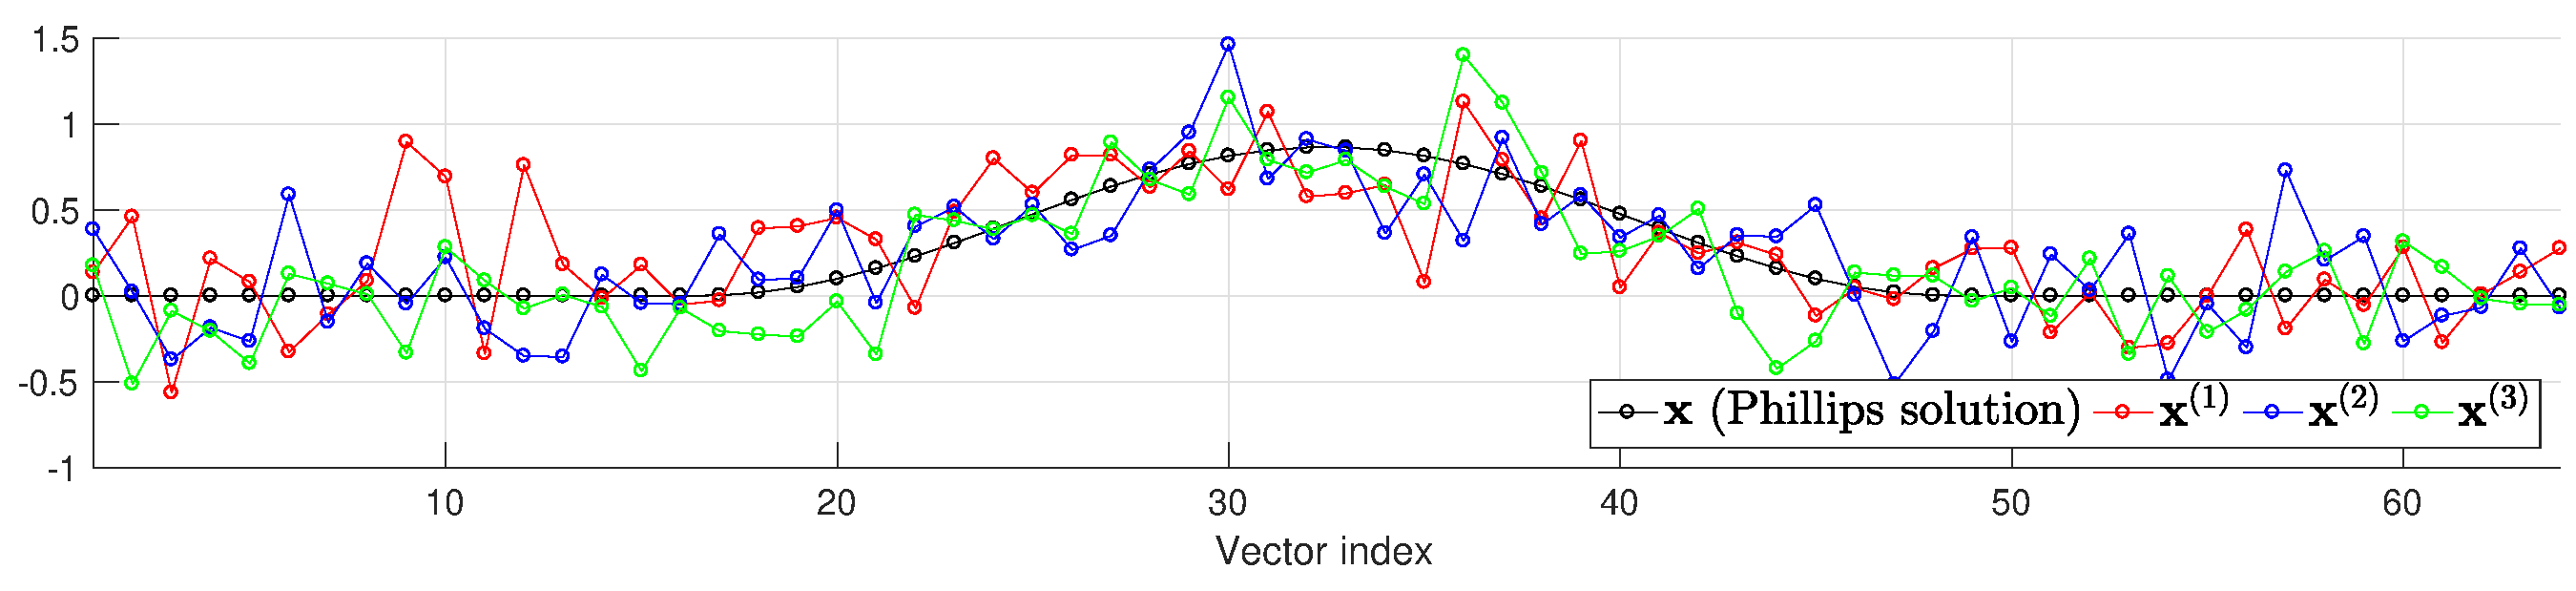
\includegraphics[scale=0.36]{Figures/Phillips-Solutions}
\subcaption{}
\end{subfigure} \\
\begin{subfigure}{\textwidth}
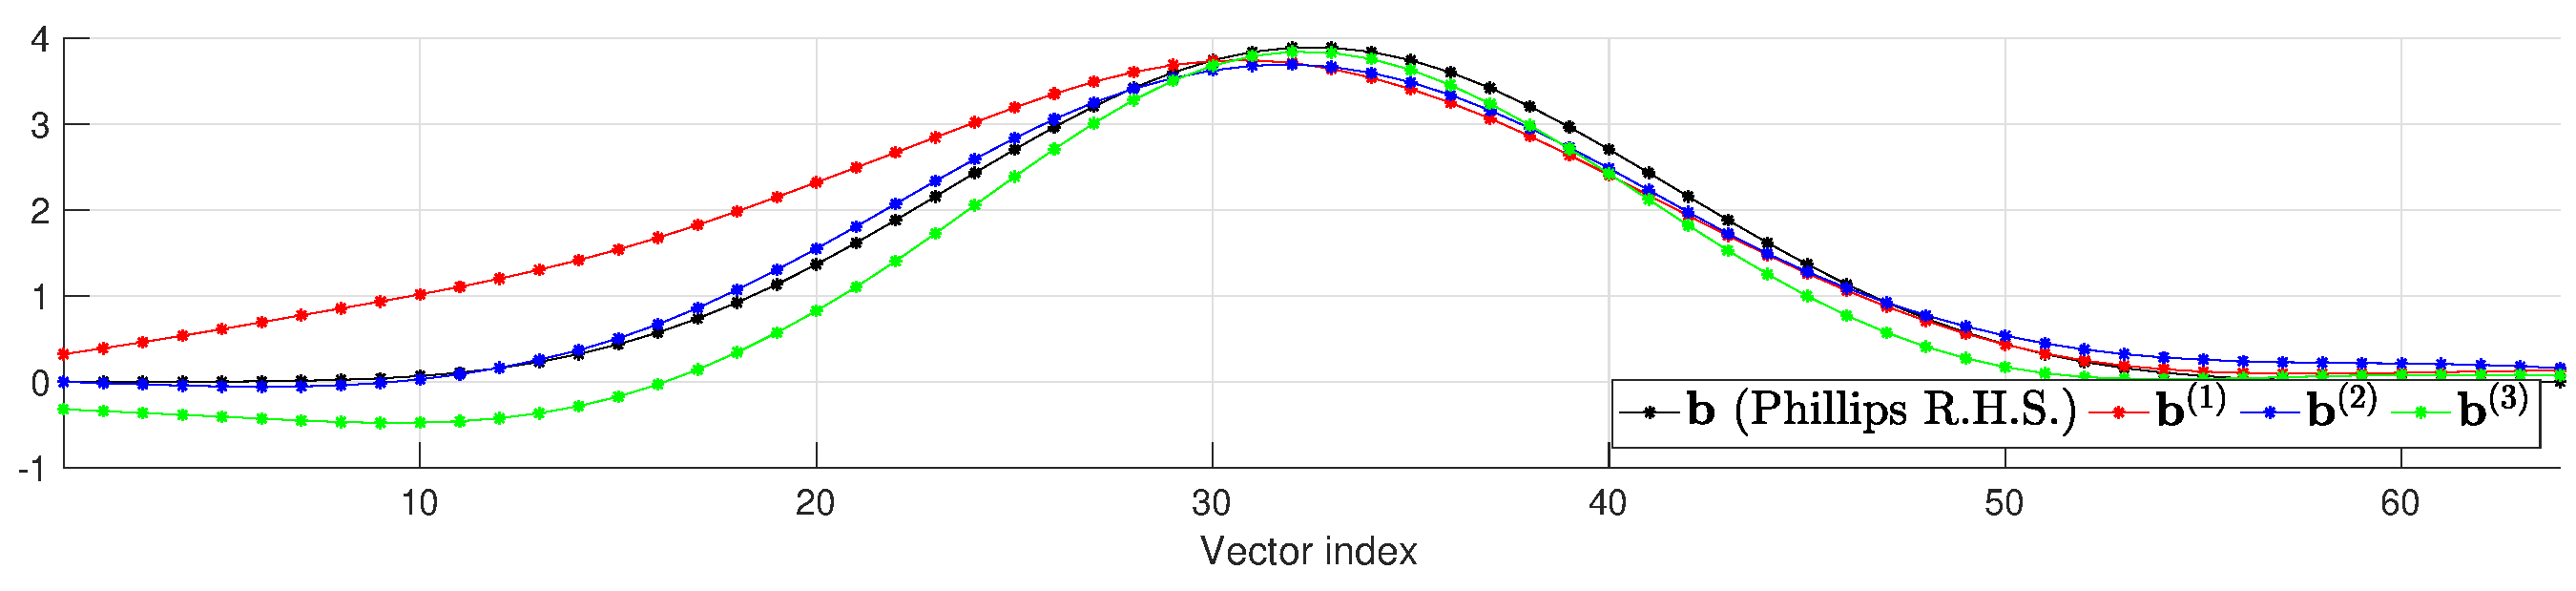
\includegraphics[scale=0.36]{Figures/Phillips-RHS}
\subcaption{}
\end{subfigure}
\caption{Examples of vectors constructed from the Phillips test problem.}
\label{fig:Phillips}
\end{figure}

%The parameters chosen by UPRE method as applied to the Phillips problem are shown in Figure \ref{fig:UPRE-Parameters-Phillips} and the corresponding errors of regularized solutions are shown in Figure \ref{fig:UPRE-Errors-Phillips}. One observation is that the parameters chosen from the adapted systems approach the mean of the parameters rapidly as the number of data sets $R$ increases. Another observation is that the range from the minimum parameter and median can be large, e.g. in the case of $n = 32$. This demonstrates the shallowness that can be characteristic of the UPRE functions which then can result is choosing the regularization parameter too small; a consequence is that the corresponding errors can be excessively large.
%
%\begin{figure}[ht]
%\begin{subfigure}{\textwidth}
%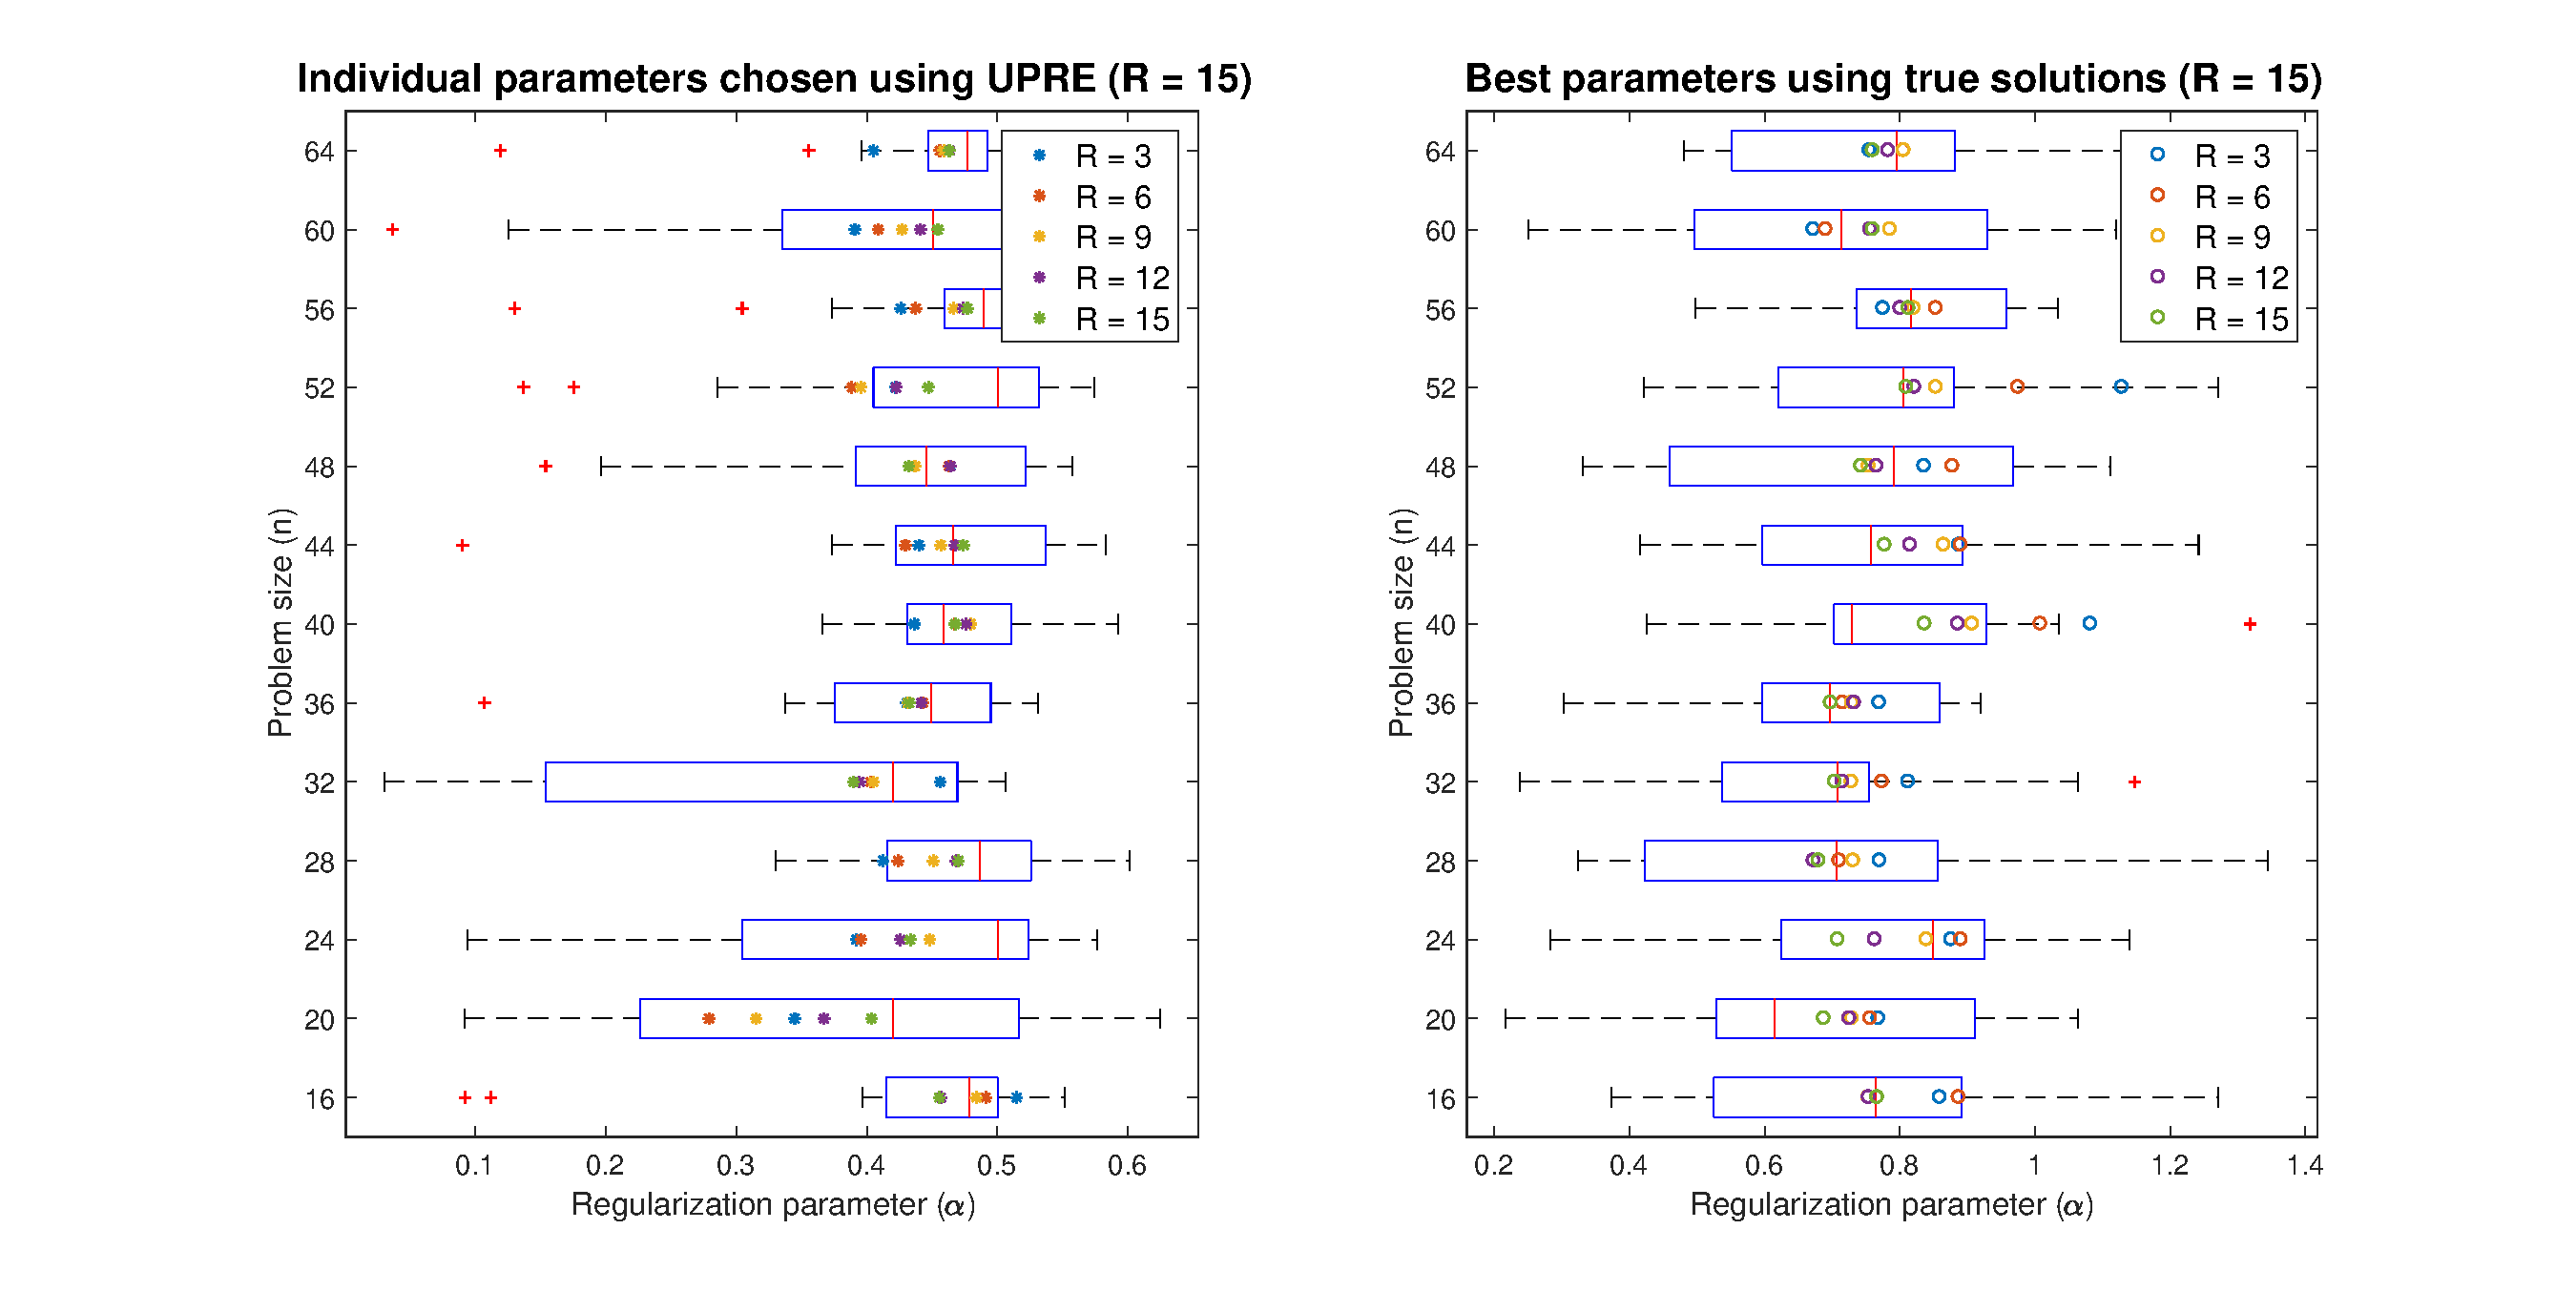
\includegraphics[scale=0.36]{Figures/UPRE-Parameters-Phillips.eps}
%\caption{Boxplots comparing the parameters chosen with the UPRE method applied to the Phillips problem.}
%\label{fig:UPRE-Parameters-Phillips}
%\end{subfigure}
%\begin{subfigure}{\textwidth}
%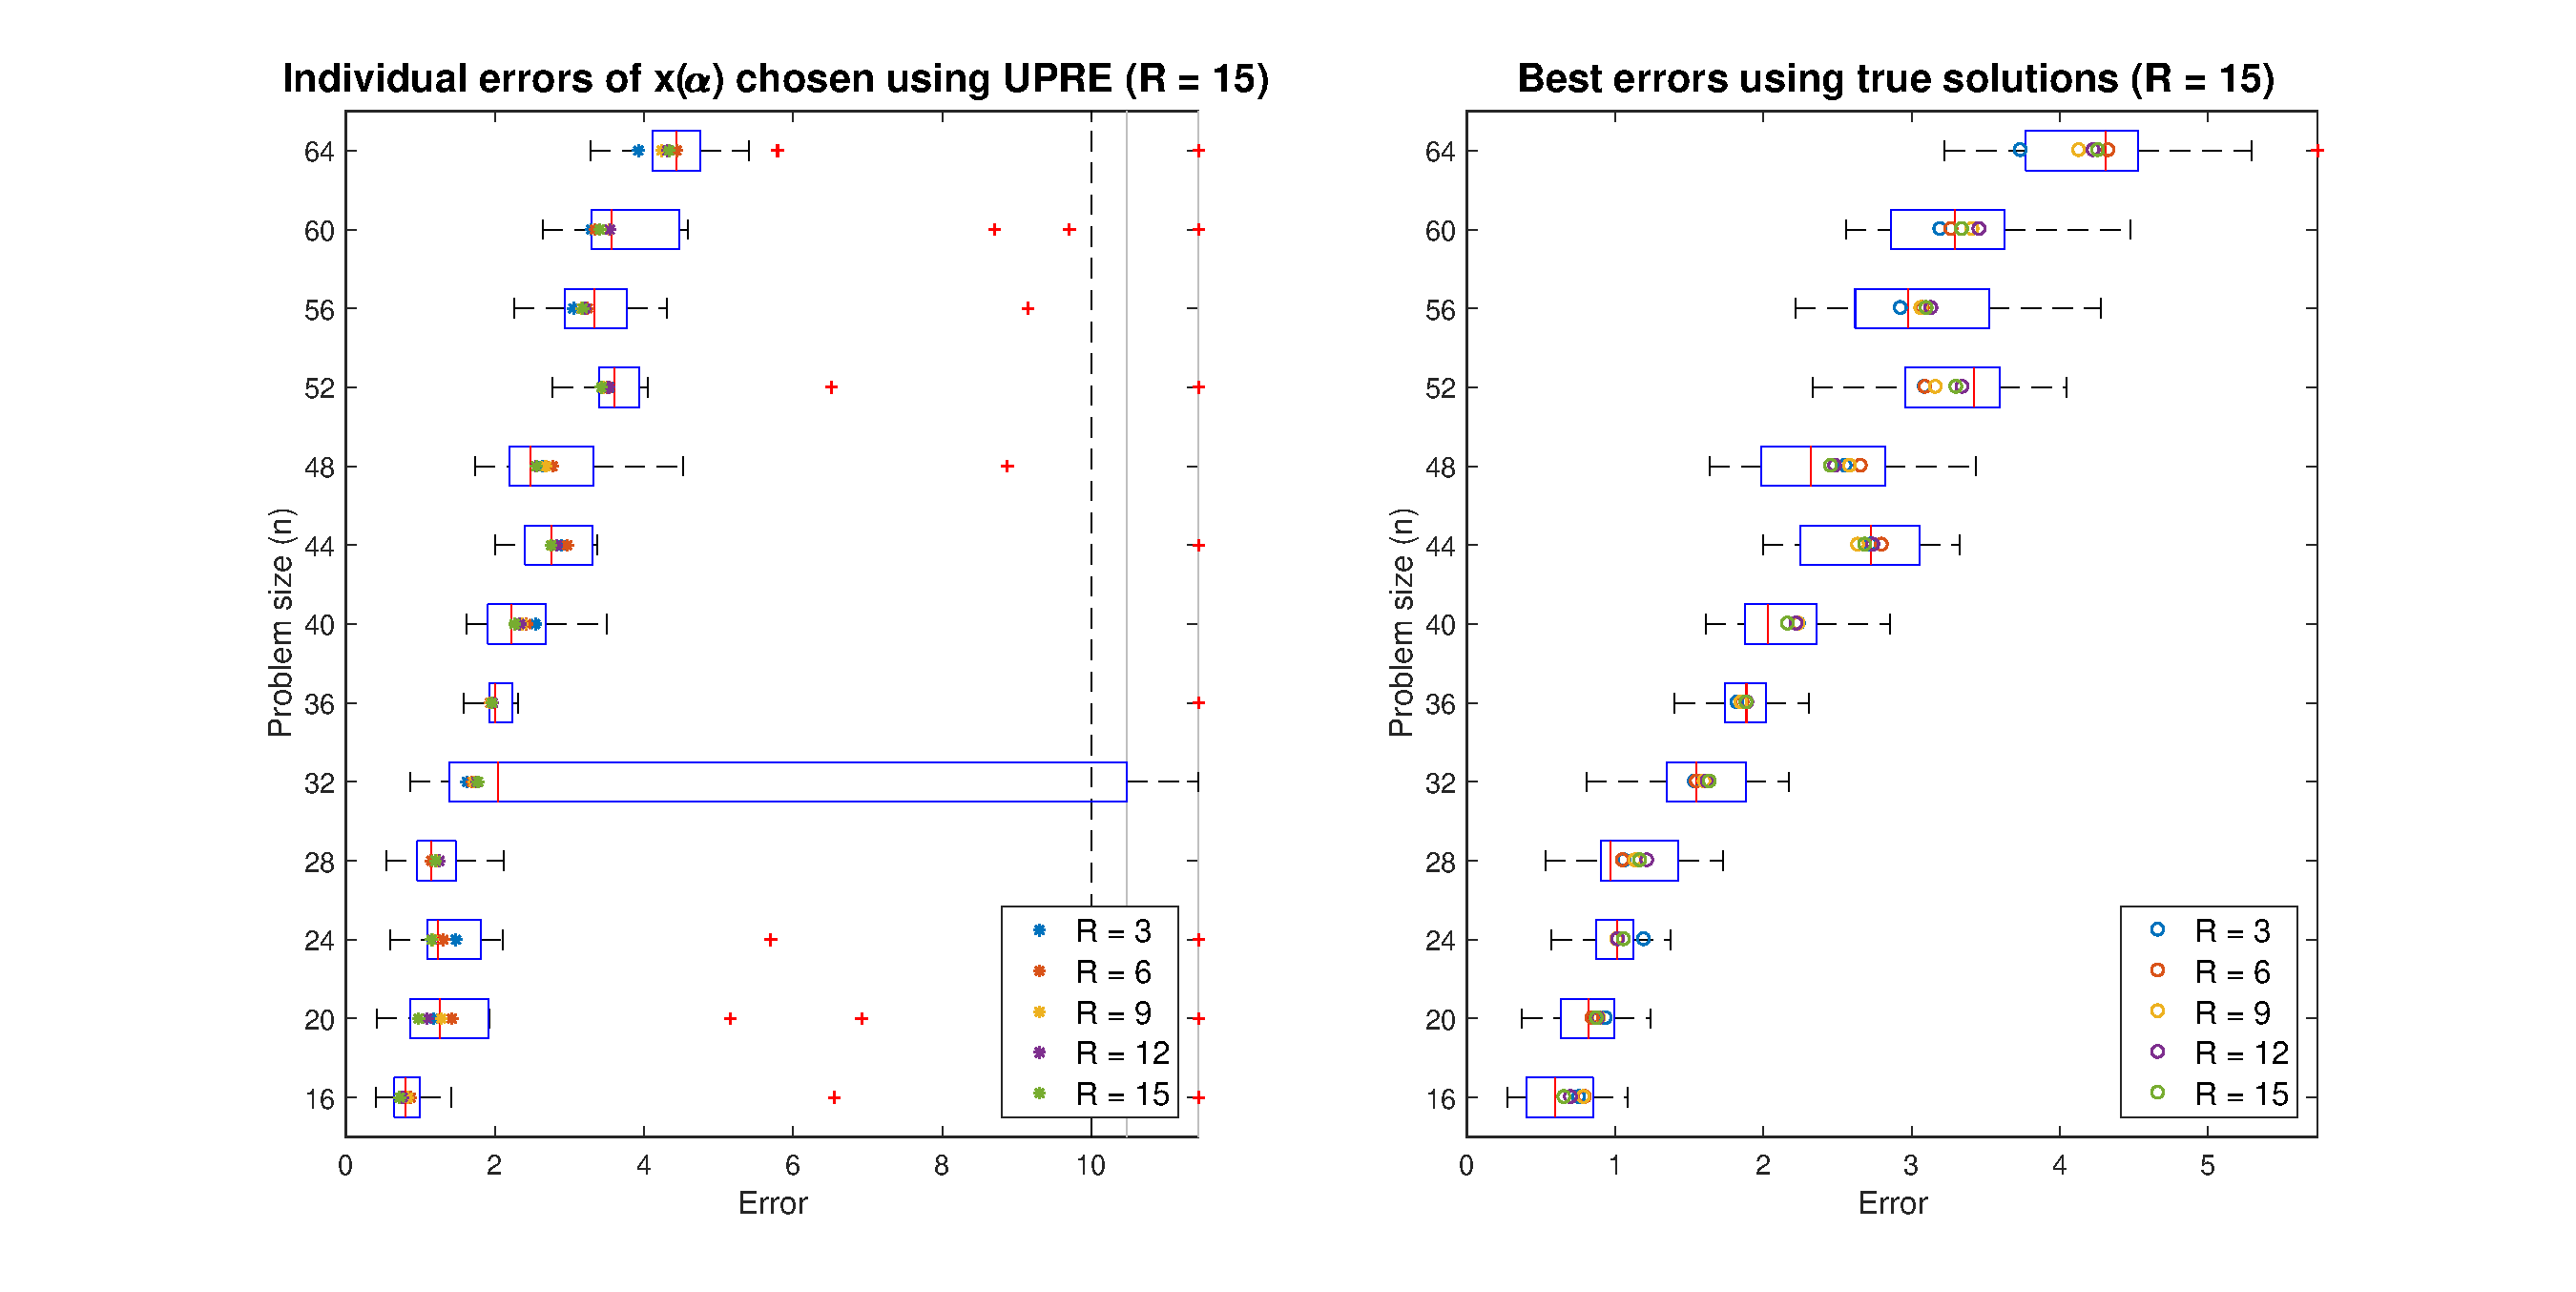
\includegraphics[scale=0.36]{Figures/UPRE-Errors-Phillips.eps}
%\caption{Boxplots comparing the errors of the regularized solutions using the parameters from the UPRE method for the Phillips problems.}
%\label{fig:UPRE-Errors-Phillips}
%\end{subfigure}
%\end{figure}
%
%\begin{figure}[ht]
%\begin{subfigure}{\textwidth}
%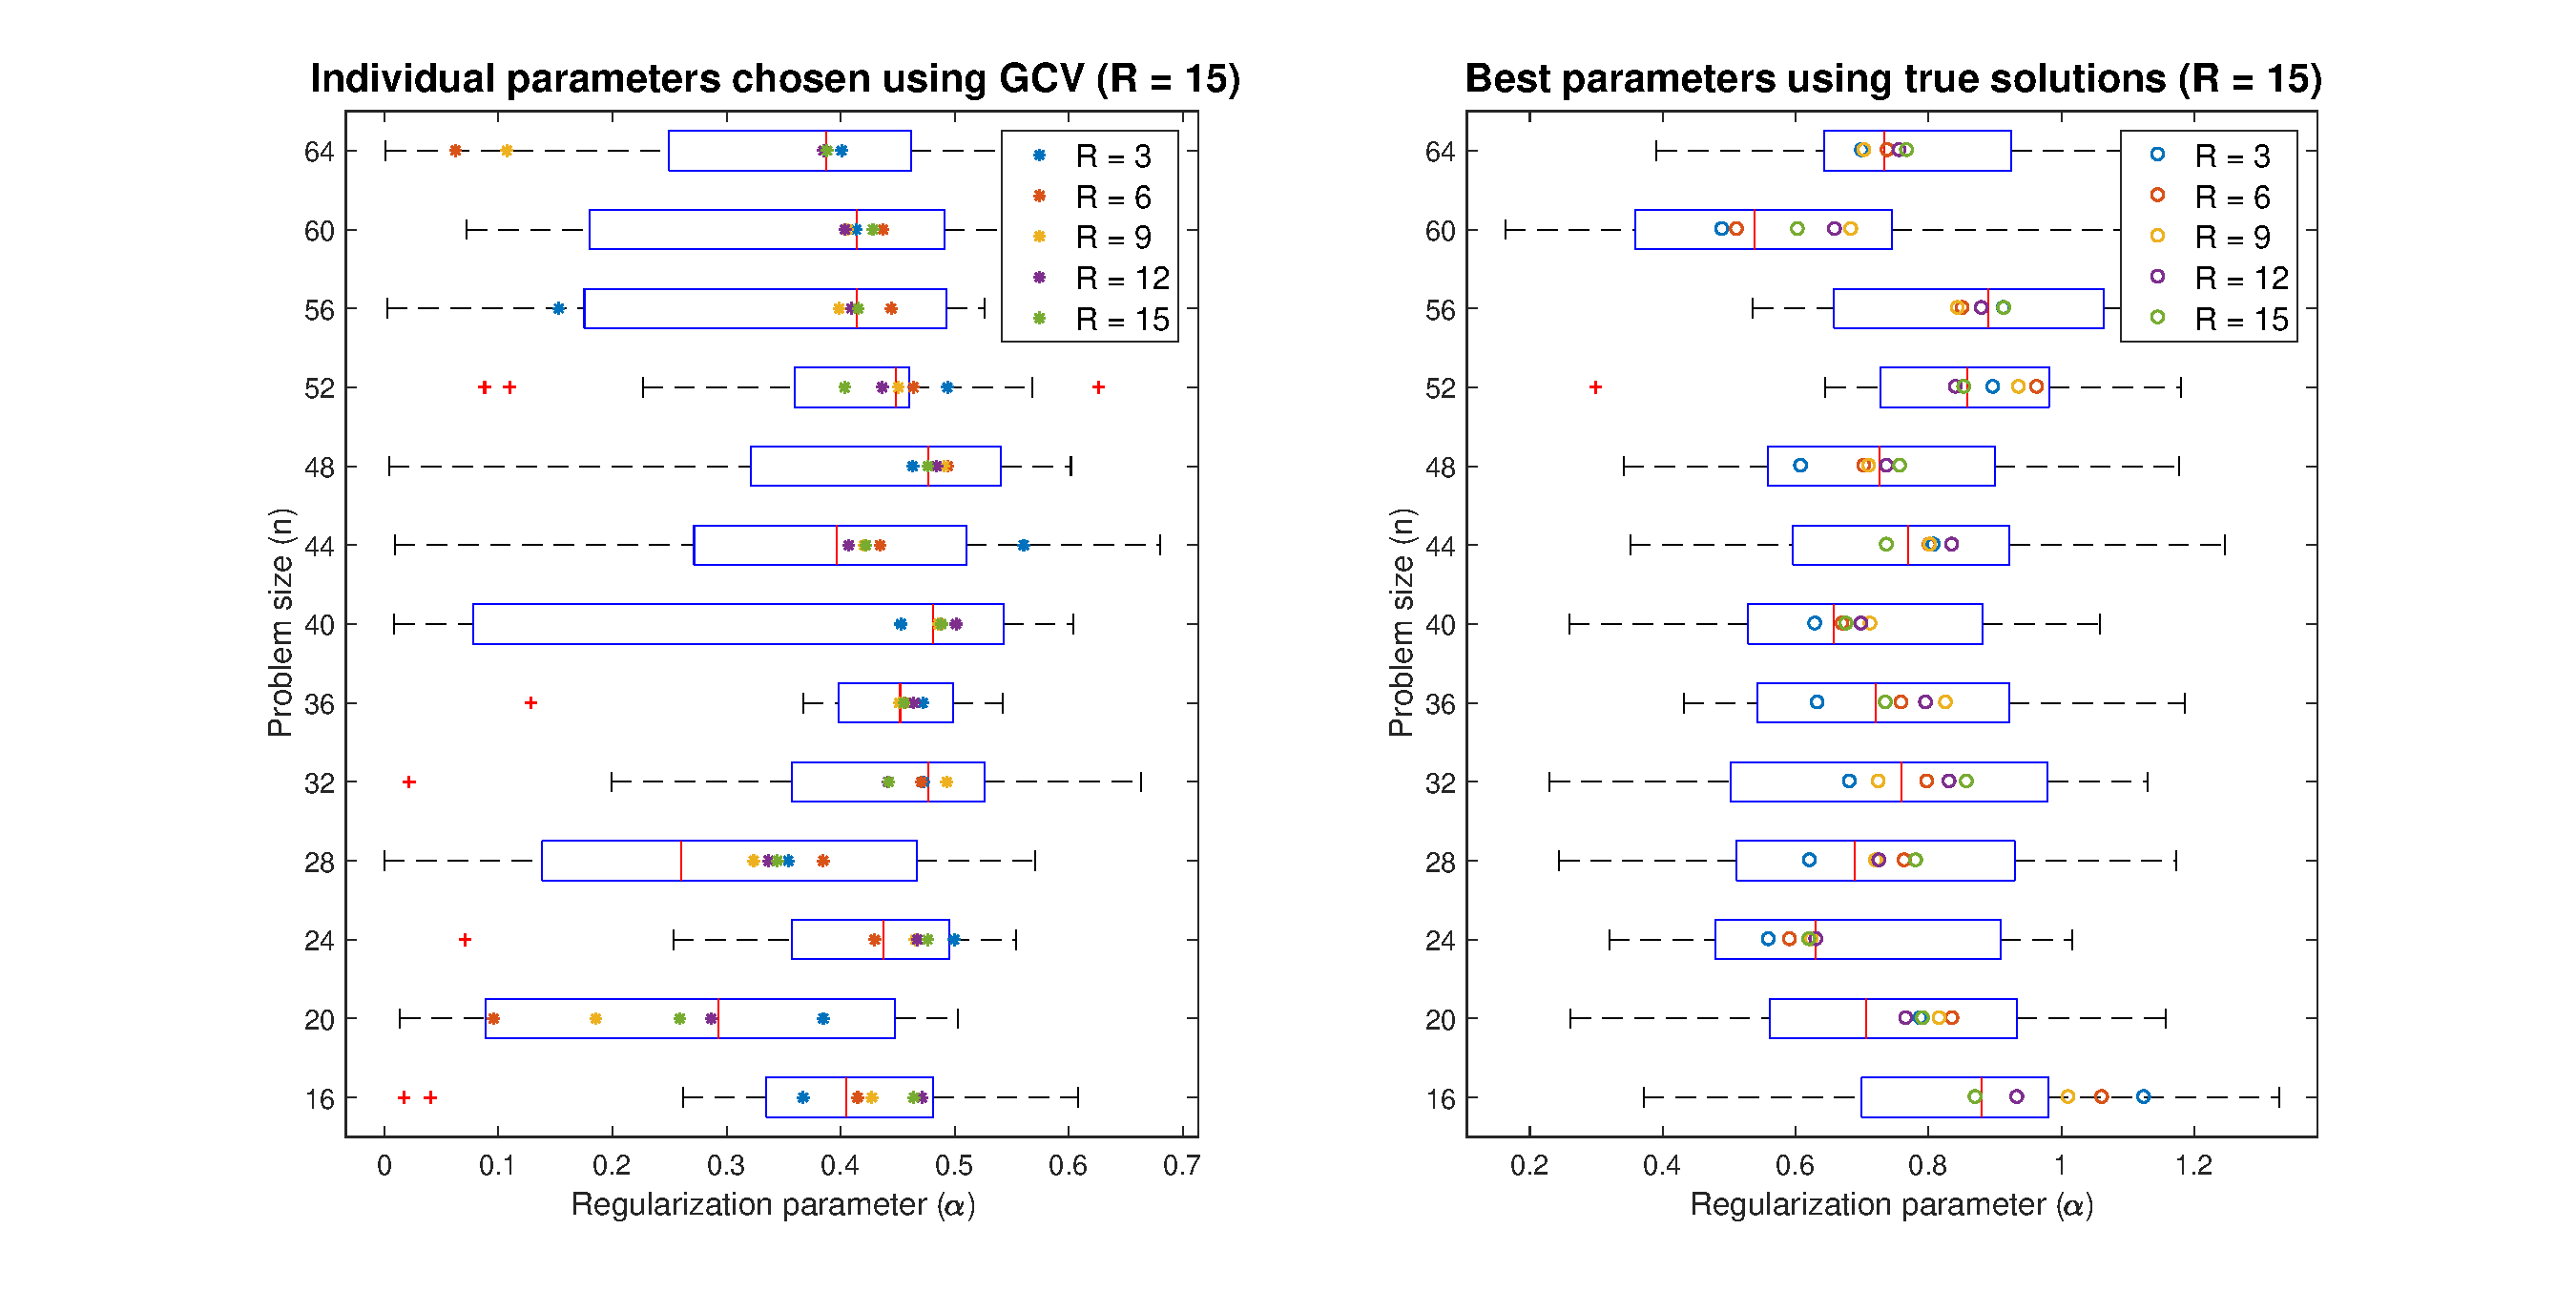
\includegraphics[scale=0.36]{Figures/GCV-Parameters-Phillips.eps}
%\caption{Boxplots comparing the parameters chosen with the GCV method applied to the Phillips problem.}
%\label{fig:GCV-Parameters-Phillips}
%\end{subfigure}
%\begin{subfigure}{\textwidth}
%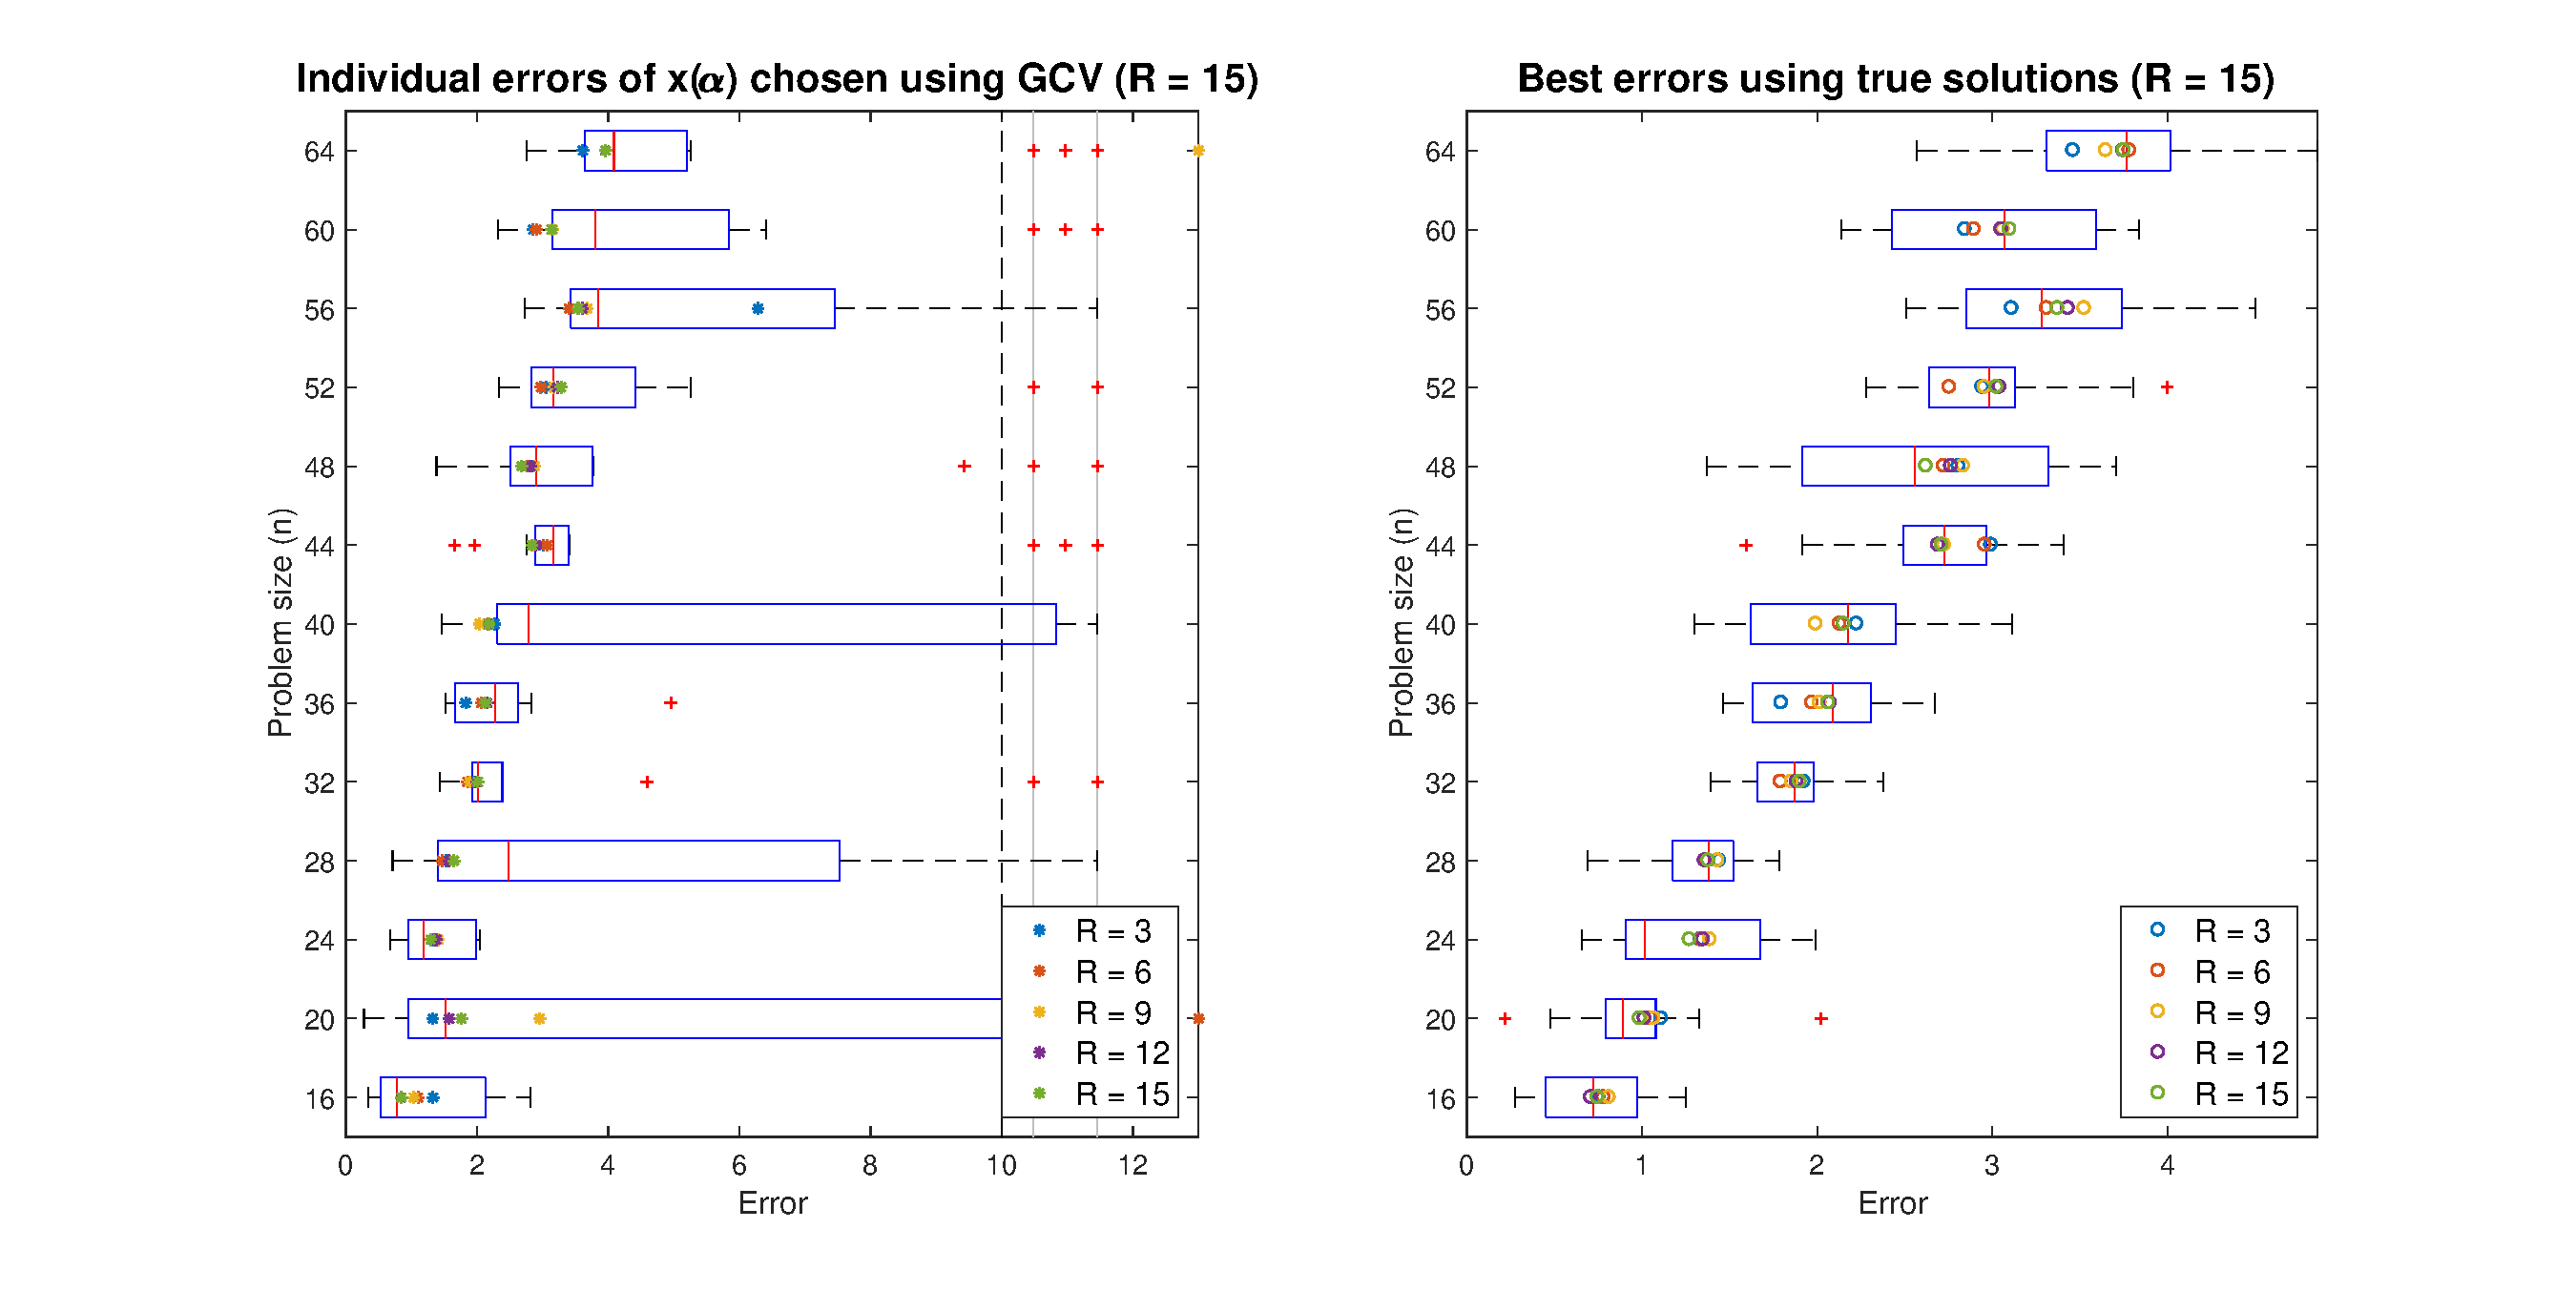
\includegraphics[scale=0.36]{Figures/GCV-Errors-Phillips.eps}
%\caption{Boxplots comparing the errors of the regularized solutions using the parameters from the GCV method for the Phillips problems.}
%\label{fig:GCV-Errors-Phillips}
%\end{subfigure}
%\end{figure}


\subsection{Two-dimensional problems} \label{sec:2D}
The second one-dimensional test problem uses the MRI data built into MATLAB, which can be accessed by the command \texttt{load mri.mat}. The built-in data was reformatted as a single image, which is a trimmed concatenation of five consecutive horizontal slices. The columns of this image were then circularly convolved with a Gaussian kernel of variance 0.01. The full sequence of MRI data and the blurred image sequence area shown in Figure \ref{fig:MRI 1D}. Since circular convolution was utilized, the DFT was the primary tool for the MRI test problem. In contrast, the SVD was used for the Phillips problem.

\begin{figure}[ht]
\begin{subfigure}{\textwidth}
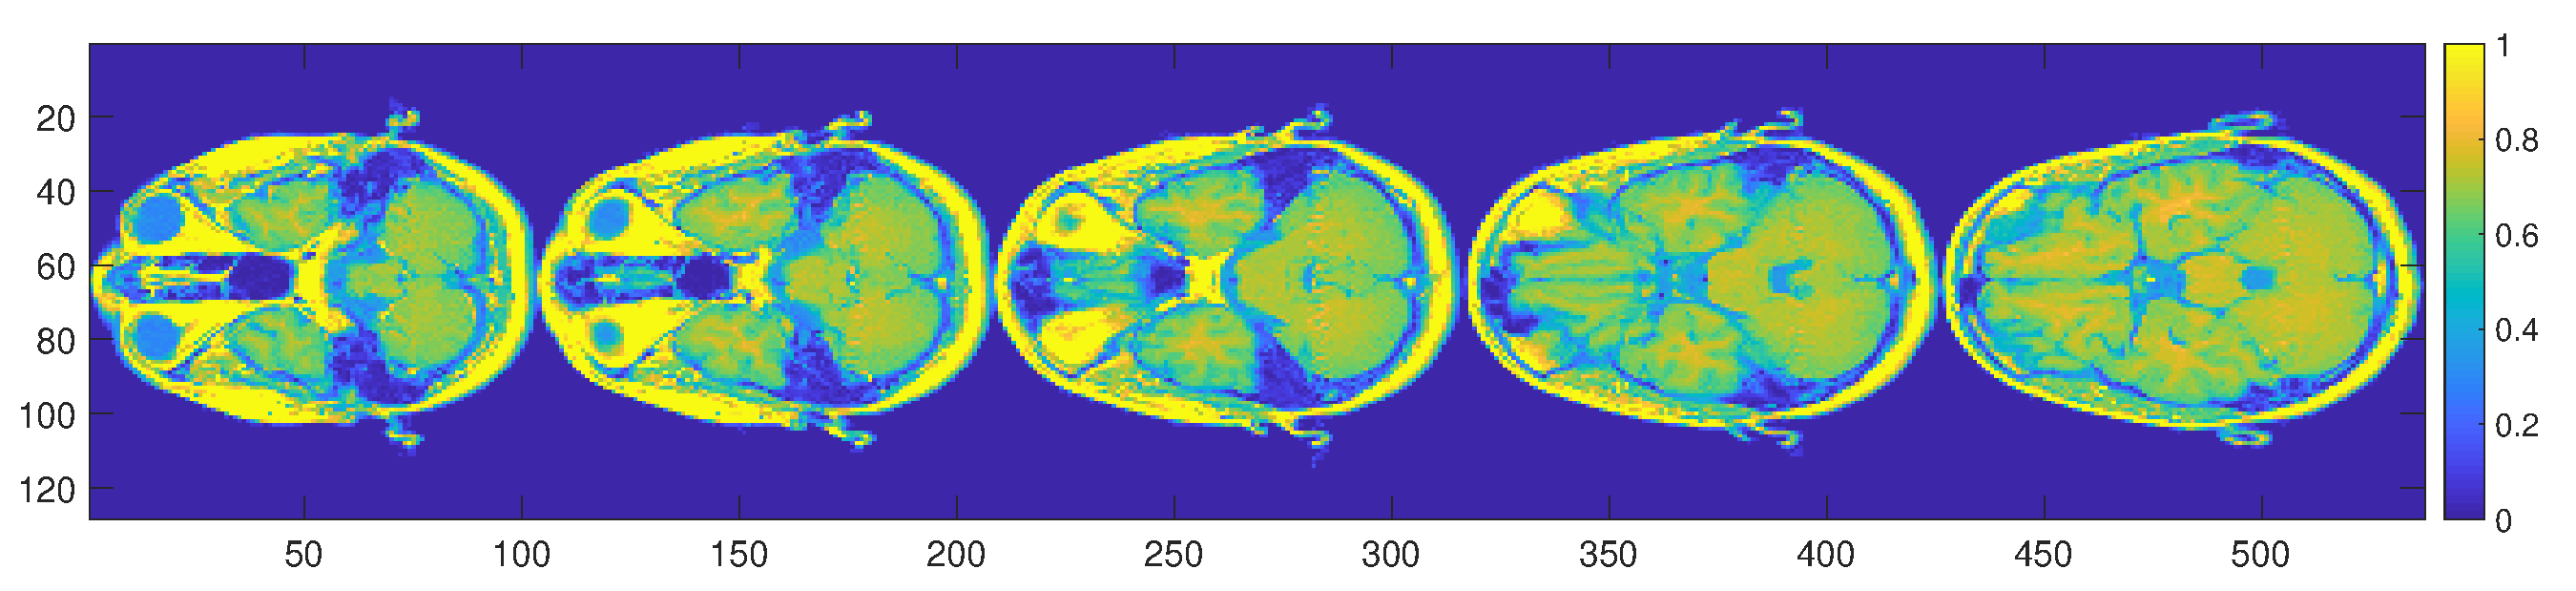
\includegraphics[scale=0.36]{Figures/Full-MRI}
\subcaption{}
\end{subfigure} \\
\begin{subfigure}{\textwidth}
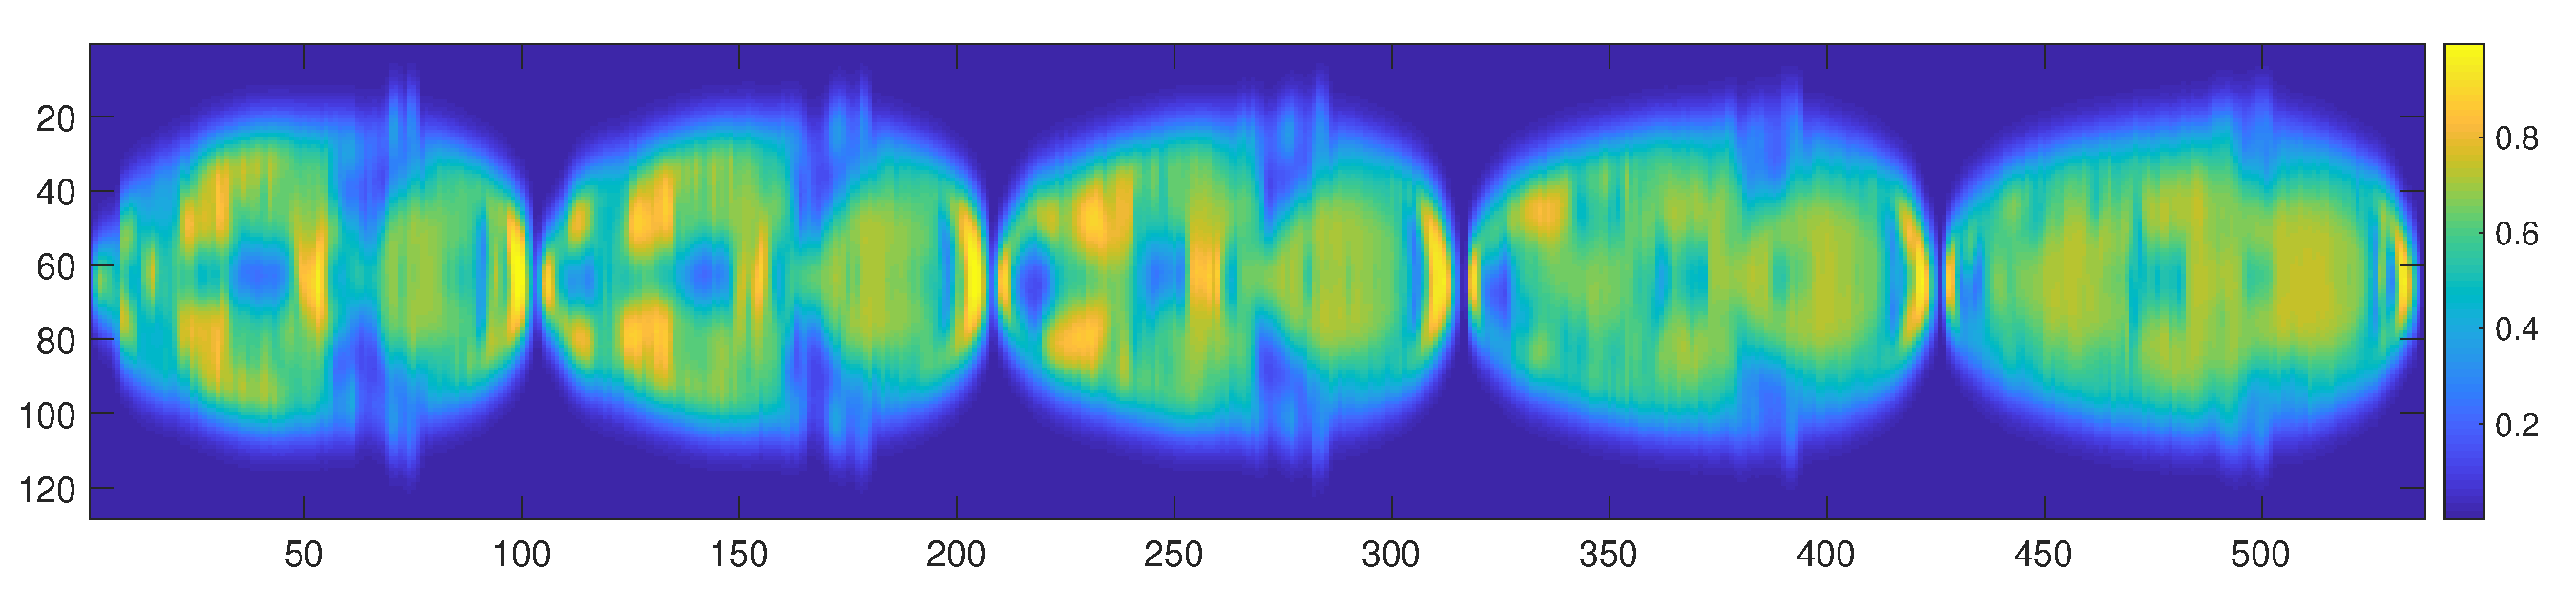
\includegraphics[scale=0.36]{Figures/Blurred-MRI}
\subcaption{}
\end{subfigure}
\caption{MRI data}
\label{fig:MRI 1D}
\end{figure}


  



%In \cite{ChungEspanol2017}, a penalty matrix selected was the following $(n+1) \times n$ matrix discretization of a first derivative operator:
%\begin{equation}
%\label{eq:Chung L}
%L = \begin{bmatrix}
%1 & & & \\
%-1 & 1 & & \\
% & \ddots & \ddots & \\
% & & -1 & 1 \\
% & & & -1
%\end{bmatrix}.
%\end{equation}
%Since the DFT is our primary tool for data processing, an assumption of periodic boundary conditions is natural and result in the square penalty matrix
%\begin{equation}
%\label{eq:Periodic L}
%L = \begin{bmatrix}
%1 & & & -1 \\
%-1 & 1 & & \\
% & \ddots & \ddots & \\
% & & -1 & 1 
%\end{bmatrix}
%\end{equation}
%as a matrix discretization of a first derivative operator. The matrix $L$ defined by \eqref{eq:Periodic L} is circulant and thus diagonalized by the unitary DFT matrix $F$. Writing $L = \ctrans{F}\Lambda{F}$, we have that $\Lambda = \diag(\sqrt{n}\dft{\mathbf{c}})$ where $\mathbf{c}$ is the first column of $L$.

\bibliographystyle{siam}
\bibliography{Parameter-Estimation}

\end{document}
